% !TEX root = ../my-thesis.tex
%
\chapter{Appendix}
\label{sec:appendix}

\section{Signals in the \(\met + V\) search}
\label{sec:appendix:monoV:signals}
The lists of \(A/V\) simplified model signal samples used for the \(\met + V\) analysis are shown in \Cref{tab:appendix:monoV:dmsimp-w} and \Cref{tab:appendix:monoV:dmsimp-z}.

\begin{table}[htb]
\caption{List is simulated signal samples of the vector mediator simplified model with \(\met + \PW\) final state}
\label{tab:appendix:monoV:dmsimp-w}
\begin{tabular}{ccccccc}
\toprule \\
signal model & process & \mZp & \mchi & \gZp & \gchi & cross-section [pb] \\
\midrule \\
\(A/V\) & \(\met + \PW\) & \SI{10}{\giga\electronvolt} & \SI{1}{\giga\electronvolt} & 0.25 & 1.0 & 338 \\
\(A/V\) & \(\met + \PW\) & \SI{100}{\giga\electronvolt} & \SI{1}{\giga\electronvolt} & 0.25 & 1.0 & 13.2 \\
\(A/V\) & \(\met + \PW\) & \SI{200}{\giga\electronvolt} & \SI{1}{\giga\electronvolt} & 0.25 & 1.0 & 4.004458 \\
\(A/V\) & \(\met + \PW\) & \SI{300}{\giga\electronvolt} & \SI{1}{\giga\electronvolt} & 0.25 & 1.0 & 1.786563 \\
\(A/V\) & \(\met + \PW\) & \SI{400}{\giga\electronvolt} & \SI{1}{\giga\electronvolt} & 0.25 & 1.0 & 0.883492 \\
\(A/V\) & \(\met + \PW\) & \SI{500}{\giga\electronvolt} & \SI{1}{\giga\electronvolt} & 0.25 & 1.0 & 0.505352 \\
\(A/V\) & \(\met + \PW\) & \SI{600}{\giga\electronvolt} & \SI{1}{\giga\electronvolt} & 0.25 & 1.0 & 0.313210 \\
\(A/V\) & \(\met + \PW\) & \SI{700}{\giga\electronvolt} & \SI{1}{\giga\electronvolt} & 0.25 & 1.0 & 0.204125 \\
\(A/V\) & \(\met + \PW\) & \SI{800}{\giga\electronvolt} & \SI{1}{\giga\electronvolt} & 0.25 & 1.0 & 0.138035 \\
\(A/V\) & \(\met + \PW\) & \SI{900}{\giga\electronvolt} & \SI{1}{\giga\electronvolt} & 0.25 & 1.0 & 0.096144 \\
\(A/V\) & \(\met + \PW\) & \SI{1000}{\giga\electronvolt} & \SI{1}{\giga\electronvolt} & 0.25 & 1.0 & 0.068471 \\
\(A/V\) & \(\met + \PW\) & \SI{2000}{\giga\electronvolt} & \SI{1}{\giga\electronvolt} & 0.25 & 1.0 & 0.00454 \\

\(A/V\) & \(\met + \PW\) & \SI{10}{\giga\electronvolt} & \SI{10}{\giga\electronvolt} & 0.25 & 1.0 & 3.41 \\
\(A/V\) & \(\met + \PW\) & \SI{100}{\giga\electronvolt} & \SI{10}{\giga\electronvolt} & 0.25 & 1.0 & 13.2 \\
\(A/V\) & \(\met + \PW\) & \SI{10000}{\giga\electronvolt} & \SI{10}{\giga\electronvolt} & 0.25 & 1.0 & 0.00000056 \\
\(A/V\) & \(\met + \PW\) & \SI{10}{\giga\electronvolt} & \SI{50}{\giga\electronvolt} & 0.25 & 1.0 & 0.199 \\
\(A/V\) & \(\met + \PW\) & \SI{50}{\giga\electronvolt} & \SI{50}{\giga\electronvolt} & 0.25 & 1.0 & 0.199 \\
\(A/V\) & \(\met + \PW\) & \SI{95}{\giga\electronvolt} & \SI{50}{\giga\electronvolt} & 0.25 & 1.0 & 1.12 \\
\(A/V\) & \(\met + \PW\) & \SI{300}{\giga\electronvolt} & \SI{50}{\giga\electronvolt} & 0.25 & 1.0 & 1.78 \\
\(A/V\) & \(\met + \PW\) & \SI{10}{\giga\electronvolt} & \SI{150}{\giga\electronvolt} & 0.25 & 1.0 & 0.0189 \\
\(A/V\) & \(\met + \PW\) & \SI{295}{\giga\electronvolt} & \SI{150}{\giga\electronvolt} & 0.25 & 1.0 & 0.263 \\
\(A/V\) & \(\met + \PW\) & \SI{1000}{\giga\electronvolt} & \SI{150}{\giga\electronvolt} & 0.25 & 1.0 & 0.068 \\
\(A/V\) & \(\met + \PW\) & \SI{10}{\giga\electronvolt} & \SI{500}{\giga\electronvolt} & 0.25 & 1.0 & 0.000457 \\
\(A/V\) & \(\met + \PW\) & \SI{995}{\giga\electronvolt} & \SI{500}{\giga\electronvolt} & 0.25 & 1.0 & 0.0143 \\
\(A/V\) & \(\met + \PW\) & \SI{2000}{\giga\electronvolt} & \SI{500}{\giga\electronvolt} & 0.25 & 1.0 & 0.00427 \\
\(A/V\) & \(\met + \PW\) & \SI{10000}{\giga\electronvolt} & \SI{500}{\giga\electronvolt} & 0.25 & 1.0 & 0.000000298 \\
\(A/V\) & \(\met + \PW\) & \SI{10}{\giga\electronvolt} & \SI{1000}{\giga\electronvolt} & 0.25 & 1.0 & 0.0000176 \\
\(A/V\) & \(\met + \PW\) & \SI{1000}{\giga\electronvolt} & \SI{100}{\giga\electronvolt} & 0.25 & 1.0 & 0.0000259 \\
\(A/V\) & \(\met + \PW\) & \SI{1995}{\giga\electronvolt} & \SI{1000}{\giga\electronvolt} & 0.25 & 1.0 & 0.000915 \\
\bottomrule
\end{tabular}
\end{table}

\begin{table}[htb]
\caption{List is simulated signal samples of the vector mediator simplified model with \(\met + \PZ\) final state}
\label{tab:appendix:monoV:dmsimp-z}
\begin{tabular}{ccccccc}
\toprule \\
signal model & process & \mZp & \mchi & \gZp & \gchi & cross-section [pb] \\
\midrule \\
\(A/V\) & \(\met + \PZ\) & \SI{10}{\giga\electronvolt} & \SI{1}{\giga\electronvolt} & 0.25 & 1.0 & 118 \\
\(A/V\) & \(\met + \PZ\) & \SI{100}{\giga\electronvolt} & \SI{1}{\giga\electronvolt} & 0.25 & 1.0 & 4.78 \\
\(A/V\) & \(\met + \PZ\) & \SI{200}{\giga\electronvolt} & \SI{1}{\giga\electronvolt} & 0.25 & 1.0 & 1.445875 \\
\(A/V\) & \(\met + \PZ\) & \SI{300}{\giga\electronvolt} & \SI{1}{\giga\electronvolt} & 0.25 & 1.0 & 0.647174 \\
\(A/V\) & \(\met + \PZ\) & \SI{400}{\giga\electronvolt} & \SI{1}{\giga\electronvolt} & 0.25 & 1.0 & 0.321675 \\
\(A/V\) & \(\met + \PZ\) & \SI{500}{\giga\electronvolt} & \SI{1}{\giga\electronvolt} & 0.25 & 1.0 & 0.184379 \\
\(A/V\) & \(\met + \PZ\) & \SI{600}{\giga\electronvolt} & \SI{1}{\giga\electronvolt} & 0.25 & 1.0 & 0.114358 \\
\(A/V\) & \(\met + \PZ\) & \SI{700}{\giga\electronvolt} & \SI{1}{\giga\electronvolt} & 0.25 & 1.0 & 0.074601 \\
\(A/V\) & \(\met + \PZ\) & \SI{800}{\giga\electronvolt} & \SI{1}{\giga\electronvolt} & 0.25 & 1.0 & 0.050488 \\
\(A/V\) & \(\met + \PZ\) & \SI{900}{\giga\electronvolt} & \SI{1}{\giga\electronvolt} & 0.25 & 1.0 & 0.035126 \\
\(A/V\) & \(\met + \PZ\) & \SI{1000}{\giga\electronvolt} & \SI{1}{\giga\electronvolt} & 0.25 & 1.0 & 0.024989 \\
\(A/V\) & \(\met + \PZ\) & \SI{2000}{\giga\electronvolt} & \SI{1}{\giga\electronvolt} & 0.25 & 1.0 & 0.00164 \\

\(A/V\) & \(\met + \PZ\) & \SI{10}{\giga\electronvolt} & \SI{10}{\giga\electronvolt} & 0.25 & 1.0 & 1.23 \\
\(A/V\) & \(\met + \PZ\) & \SI{100}{\giga\electronvolt} & \SI{10}{\giga\electronvolt} & 0.25 & 1.0 & 4.77 \\
\(A/V\) & \(\met + \PZ\) & \SI{10000}{\giga\electronvolt} & \SI{10}{\giga\electronvolt} & 0.25 & 1.0 & 0.000000193 \\
\(A/V\) & \(\met + \PZ\) & \SI{10}{\giga\electronvolt} & \SI{50}{\giga\electronvolt} & 0.25 & 1.0 & 0.0717 \\
\(A/V\) & \(\met + \PZ\) & \SI{95}{\giga\electronvolt} & \SI{50}{\giga\electronvolt} & 0.25 & 1.0 & 0.404 \\
\(A/V\) & \(\met + \PZ\) & \SI{300}{\giga\electronvolt} & \SI{50}{\giga\electronvolt} & 0.25 & 1.0 & 0.645 \\
\(A/V\) & \(\met + \PZ\) & \SI{10}{\giga\electronvolt} & \SI{150}{\giga\electronvolt} & 0.25 & 1.0 & 0.00690 \\
\(A/V\) & \(\met + \PZ\) & \SI{295}{\giga\electronvolt} & \SI{150}{\giga\electronvolt} & 0.25 & 1.0 & 0.0955 \\
\(A/V\) & \(\met + \PZ\) & \SI{1000}{\giga\electronvolt} & \SI{150}{\giga\electronvolt} & 0.25 & 1.0 & 0.0248 \\
\(A/V\) & \(\met + \PZ\) & \SI{10}{\giga\electronvolt} & \SI{500}{\giga\electronvolt} & 0.25 & 1.0 & 0.000166 \\
\(A/V\) & \(\met + \PZ\) & \SI{995}{\giga\electronvolt} & \SI{500}{\giga\electronvolt} & 0.25 & 1.0 & 0.00523 \\
\(A/V\) & \(\met + \PZ\) & \SI{2000}{\giga\electronvolt} & \SI{500}{\giga\electronvolt} & 0.25 & 1.0 & 0.00154 \\
\(A/V\) & \(\met + \PZ\) & \SI{10000}{\giga\electronvolt} & \SI{500}{\giga\electronvolt} & 0.25 & 1.0 & 0.000000110 \\
\(A/V\) & \(\met + \PZ\) & \SI{10}{\giga\electronvolt} & \SI{1000}{\giga\electronvolt} & 0.25 & 1.0 & 0.00000646 \\
\(A/V\) & \(\met + \PZ\) & \SI{1000}{\giga\electronvolt} & \SI{100}{\giga\electronvolt} & 0.25 & 1.0 & 0.00000948 \\
\(A/V\) & \(\met + \PZ\) & \SI{1995}{\giga\electronvolt} & \SI{1000}{\giga\electronvolt} & 0.25 & 1.0 & 0.000330 \\
\bottomrule
\end{tabular}
\end{table}




\begin{table}[htb]
\caption{List is simulated signal samples of the \ahdm simplified model with \(\met + \PZ\) final state}
\label{tab:appendix:monoV:ahdm-z1}
\begin{tabular}{cccccc}
\toprule \\
signal model & process & \(\tan \beta\) & \mA & \ma & \mchi \\
\midrule \\
\ahdm & \(\met + \PZ\) & \num{1.0} & \SI{200}{\giga\electronvolt} & \SI{100}{\giga\electronvolt} & \SI{10}{\giga\electronvolt} \\
\ahdm & \(\met + \PZ\) & \num{1.0} & \SI{250}{\giga\electronvolt} & \SI{100}{\giga\electronvolt} & \SI{10}{\giga\electronvolt} \\
\ahdm & \(\met + \PZ\) & \num{1.0} & \SI{250}{\giga\electronvolt} & \SI{150}{\giga\electronvolt} & \SI{10}{\giga\electronvolt} \\
\ahdm & \(\met + \PZ\) & \num{1.0} & \SI{300}{\giga\electronvolt} & \SI{100}{\giga\electronvolt} & \SI{10}{\giga\electronvolt} \\
\ahdm & \(\met + \PZ\) & \num{1.0} & \SI{300}{\giga\electronvolt} & \SI{150}{\giga\electronvolt} & \SI{10}{\giga\electronvolt} \\
\ahdm & \(\met + \PZ\) & \num{1.0} & \SI{300}{\giga\electronvolt} & \SI{200}{\giga\electronvolt} & \SI{10}{\giga\electronvolt} \\
\ahdm & \(\met + \PZ\) & \num{1.0} & \SI{300}{\giga\electronvolt} & \SI{250}{\giga\electronvolt} & \SI{10}{\giga\electronvolt} \\
\ahdm & \(\met + \PZ\) & \num{1.0} & \SI{350}{\giga\electronvolt} & \SI{200}{\giga\electronvolt} & \SI{10}{\giga\electronvolt} \\
\ahdm & \(\met + \PZ\) & \num{1.0} & \SI{350}{\giga\electronvolt} & \SI{250}{\giga\electronvolt} & \SI{10}{\giga\electronvolt} \\
\ahdm & \(\met + \PZ\) & \num{1.0} & \SI{350}{\giga\electronvolt} & \SI{300}{\giga\electronvolt} & \SI{10}{\giga\electronvolt} \\
\ahdm & \(\met + \PZ\) & \num{1.0} & \SI{400}{\giga\electronvolt} & \SI{100}{\giga\electronvolt} & \SI{10}{\giga\electronvolt} \\
\ahdm & \(\met + \PZ\) & \num{1.0} & \SI{400}{\giga\electronvolt} & \SI{150}{\giga\electronvolt} & \SI{10}{\giga\electronvolt} \\
\ahdm & \(\met + \PZ\) & \num{1.0} & \SI{400}{\giga\electronvolt} & \SI{200}{\giga\electronvolt} & \SI{10}{\giga\electronvolt} \\
\ahdm & \(\met + \PZ\) & \num{1.0} & \SI{400}{\giga\electronvolt} & \SI{250}{\giga\electronvolt} & \SI{10}{\giga\electronvolt} \\
\ahdm & \(\met + \PZ\) & \num{1.0} & \SI{400}{\giga\electronvolt} & \SI{300}{\giga\electronvolt} & \SI{10}{\giga\electronvolt} \\
\ahdm & \(\met + \PZ\) & \num{1.0} & \SI{400}{\giga\electronvolt} & \SI{350}{\giga\electronvolt} & \SI{10}{\giga\electronvolt} \\
\ahdm & \(\met + \PZ\) & \num{1.0} & \SI{500}{\giga\electronvolt} & \SI{100}{\giga\electronvolt} & \SI{10}{\giga\electronvolt} \\
\ahdm & \(\met + \PZ\) & \num{1.0} & \SI{500}{\giga\electronvolt} & \SI{150}{\giga\electronvolt} & \SI{10}{\giga\electronvolt} \\
\ahdm & \(\met + \PZ\) & \num{1.0} & \SI{500}{\giga\electronvolt} & \SI{200}{\giga\electronvolt} & \SI{10}{\giga\electronvolt} \\
\ahdm & \(\met + \PZ\) & \num{1.0} & \SI{500}{\giga\electronvolt} & \SI{250}{\giga\electronvolt} & \SI{10}{\giga\electronvolt} \\
\ahdm & \(\met + \PZ\) & \num{1.0} & \SI{500}{\giga\electronvolt} & \SI{300}{\giga\electronvolt} & \SI{10}{\giga\electronvolt} \\
\ahdm & \(\met + \PZ\) & \num{1.0} & \SI{500}{\giga\electronvolt} & \SI{350}{\giga\electronvolt} & \SI{10}{\giga\electronvolt} \\
\ahdm & \(\met + \PZ\) & \num{1.0} & \SI{600}{\giga\electronvolt} & \SI{100}{\giga\electronvolt} & \SI{10}{\giga\electronvolt} \\
\ahdm & \(\met + \PZ\) & \num{1.0} & \SI{600}{\giga\electronvolt} & \SI{200}{\giga\electronvolt} & \SI{10}{\giga\electronvolt} \\
\ahdm & \(\met + \PZ\) & \num{1.0} & \SI{600}{\giga\electronvolt} & \SI{300}{\giga\electronvolt} & \SI{10}{\giga\electronvolt} \\
\ahdm & \(\met + \PZ\) & \num{1.0} & \SI{600}{\giga\electronvolt} & \SI{350}{\giga\electronvolt} & \SI{10}{\giga\electronvolt} \\
\ahdm & \(\met + \PZ\) & \num{1.0} & \SI{600}{\giga\electronvolt} & \SI{400}{\giga\electronvolt} & \SI{10}{\giga\electronvolt} \\
\ahdm & \(\met + \PZ\) & \num{1.0} & \SI{700}{\giga\electronvolt} & \SI{300}{\giga\electronvolt} & \SI{10}{\giga\electronvolt} \\
\ahdm & \(\met + \PZ\) & \num{1.0} & \SI{700}{\giga\electronvolt} & \SI{350}{\giga\electronvolt} & \SI{10}{\giga\electronvolt} \\
\ahdm & \(\met + \PZ\) & \num{1.0} & \SI{700}{\giga\electronvolt} & \SI{400}{\giga\electronvolt} & \SI{10}{\giga\electronvolt} \\
\ahdm & \(\met + \PZ\) & \num{1.0} & \SI{700}{\giga\electronvolt} & \SI{500}{\giga\electronvolt} & \SI{10}{\giga\electronvolt} \\
\ahdm & \(\met + \PZ\) & \num{1.0} & \SI{800}{\giga\electronvolt} & \SI{400}{\giga\electronvolt} & \SI{10}{\giga\electronvolt} \\
\ahdm & \(\met + \PZ\) & \num{1.0} & \SI{800}{\giga\electronvolt} & \SI{400}{\giga\electronvolt} & \SI{10}{\giga\electronvolt} \\
\ahdm & \(\met + \PZ\) & \num{1.0} & \SI{800}{\giga\electronvolt} & \SI{500}{\giga\electronvolt} & \SI{10}{\giga\electronvolt} \\
\ahdm & \(\met + \PZ\) & \num{1.0} & \SI{800}{\giga\electronvolt} & \SI{500}{\giga\electronvolt} & \SI{10}{\giga\electronvolt} \\
\ahdm & \(\met + \PZ\) & \num{1.0} & \SI{900}{\giga\electronvolt} & \SI{400}{\giga\electronvolt} & \SI{10}{\giga\electronvolt} \\
\ahdm & \(\met + \PZ\) & \num{1.0} & \SI{900}{\giga\electronvolt} & \SI{500}{\giga\electronvolt} & \SI{10}{\giga\electronvolt} \\
\ahdm & \(\met + \PZ\) & \num{1.0} & \SI{1000}{\giga\electronvolt} & \SI{400}{\giga\electronvolt} & \SI{10}{\giga\electronvolt} \\
\ahdm & \(\met + \PZ\) & \num{1.0} & \SI{1000}{\giga\electronvolt} & \SI{500}{\giga\electronvolt} & \SI{10}{\giga\electronvolt} \\
\ahdm & \(\met + \PZ\) & \num{1.0} & \SI{1100}{\giga\electronvolt} & \SI{150}{\giga\electronvolt} & \SI{10}{\giga\electronvolt} \\
\ahdm & \(\met + \PZ\) & \num{1.0} & \SI{1100}{\giga\electronvolt} & \SI{250}{\giga\electronvolt} & \SI{10}{\giga\electronvolt} \\
\ahdm & \(\met + \PZ\) & \num{1.0} & \SI{1100}{\giga\electronvolt} & \SI{350}{\giga\electronvolt} & \SI{10}{\giga\electronvolt} \\
\ahdm & \(\met + \PZ\) & \num{1.0} & \SI{1100}{\giga\electronvolt} & \SI{400}{\giga\electronvolt} & \SI{10}{\giga\electronvolt} \\
\ahdm & \(\met + \PZ\) & \num{1.0} & \SI{1100}{\giga\electronvolt} & \SI{500}{\giga\electronvolt} & \SI{10}{\giga\electronvolt} \\
\ahdm & \(\met + \PZ\) & \num{1.0} & \SI{1200}{\giga\electronvolt} & \SI{150}{\giga\electronvolt} & \SI{10}{\giga\electronvolt} \\
\ahdm & \(\met + \PZ\) & \num{1.0} & \SI{1200}{\giga\electronvolt} & \SI{250}{\giga\electronvolt} & \SI{10}{\giga\electronvolt} \\
\ahdm & \(\met + \PZ\) & \num{1.0} & \SI{1200}{\giga\electronvolt} & \SI{350}{\giga\electronvolt} & \SI{10}{\giga\electronvolt} \\
\ahdm & \(\met + \PZ\) & \num{1.0} & \SI{1200}{\giga\electronvolt} & \SI{400}{\giga\electronvolt} & \SI{10}{\giga\electronvolt} \\
\ahdm & \(\met + \PZ\) & \num{1.0} & \SI{1300}{\giga\electronvolt} & \SI{150}{\giga\electronvolt} & \SI{10}{\giga\electronvolt} \\
\ahdm & \(\met + \PZ\) & \num{1.0} & \SI{1300}{\giga\electronvolt} & \SI{250}{\giga\electronvolt} & \SI{10}{\giga\electronvolt} \\
\ahdm & \(\met + \PZ\) & \num{1.0} & \SI{1300}{\giga\electronvolt} & \SI{350}{\giga\electronvolt} & \SI{10}{\giga\electronvolt} \\
\ahdm & \(\met + \PZ\) & \num{1.0} & \SI{1400}{\giga\electronvolt} & \SI{150}{\giga\electronvolt} & \SI{10}{\giga\electronvolt} \\
\ahdm & \(\met + \PZ\) & \num{1.0} & \SI{1400}{\giga\electronvolt} & \SI{250}{\giga\electronvolt} & \SI{10}{\giga\electronvolt} \\
\ahdm & \(\met + \PZ\) & \num{1.0} & \SI{1400}{\giga\electronvolt} & \SI{350}{\giga\electronvolt} & \SI{10}{\giga\electronvolt} \\
\bottomrule
\end{tabular}
\end{table}



\begin{table}[htb]
\caption{List is simulated signal samples of the \ahdm simplified model with \(\met + \PZ\) final state}
\label{tab:appendix:monoV:ahdm-z2}
\begin{tabular}{cccccc}
\toprule \\
signal model & process & \(\tan \beta\) & \mA & \ma & \mchi \\
\midrule \\
\ahdm & \(\met + \PZ\) & \num{0.3} & \SI{600}{\giga\electronvolt} & \SI{100}{\giga\electronvolt} & \SI{10}{\giga\electronvolt} \\
\ahdm & \(\met + \PZ\) & \num{0.3} & \SI{600}{\giga\electronvolt} & \SI{200}{\giga\electronvolt} & \SI{10}{\giga\electronvolt} \\
\ahdm & \(\met + \PZ\) & \num{0.3} & \SI{600}{\giga\electronvolt} & \SI{300}{\giga\electronvolt} & \SI{10}{\giga\electronvolt} \\
\ahdm & \(\met + \PZ\) & \num{0.3} & \SI{600}{\giga\electronvolt} & \SI{350}{\giga\electronvolt} & \SI{10}{\giga\electronvolt} \\
\ahdm & \(\met + \PZ\) & \num{0.3} & \SI{600}{\giga\electronvolt} & \SI{400}{\giga\electronvolt} & \SI{10}{\giga\electronvolt} \\
\ahdm & \(\met + \PZ\) & \num{0.5} & \SI{600}{\giga\electronvolt} & \SI{100}{\giga\electronvolt} & \SI{10}{\giga\electronvolt} \\
\ahdm & \(\met + \PZ\) & \num{0.5} & \SI{600}{\giga\electronvolt} & \SI{200}{\giga\electronvolt} & \SI{10}{\giga\electronvolt} \\
\ahdm & \(\met + \PZ\) & \num{0.5} & \SI{600}{\giga\electronvolt} & \SI{300}{\giga\electronvolt} & \SI{10}{\giga\electronvolt} \\
\ahdm & \(\met + \PZ\) & \num{0.5} & \SI{600}{\giga\electronvolt} & \SI{350}{\giga\electronvolt} & \SI{10}{\giga\electronvolt} \\
\ahdm & \(\met + \PZ\) & \num{0.5} & \SI{600}{\giga\electronvolt} & \SI{400}{\giga\electronvolt} & \SI{10}{\giga\electronvolt} \\
\ahdm & \(\met + \PZ\) & \num{3.0} & \SI{600}{\giga\electronvolt} & \SI{100}{\giga\electronvolt} & \SI{10}{\giga\electronvolt} \\
\ahdm & \(\met + \PZ\) & \num{3.0} & \SI{600}{\giga\electronvolt} & \SI{200}{\giga\electronvolt} & \SI{10}{\giga\electronvolt} \\
\ahdm & \(\met + \PZ\) & \num{3.0} & \SI{600}{\giga\electronvolt} & \SI{300}{\giga\electronvolt} & \SI{10}{\giga\electronvolt} \\
\ahdm & \(\met + \PZ\) & \num{3.0} & \SI{600}{\giga\electronvolt} & \SI{350}{\giga\electronvolt} & \SI{10}{\giga\electronvolt} \\
\ahdm & \(\met + \PZ\) & \num{3.0} & \SI{600}{\giga\electronvolt} & \SI{400}{\giga\electronvolt} & \SI{10}{\giga\electronvolt} \\
\bottomrule
\end{tabular}
\end{table}


\begin{table}[htb]
\caption{List is simulated signal samples of the \ahdm simplified model with \(\met + \PZ\) final state}
\label{tab:appendix:monoV:ahdm-z3}
\begin{tabular}{cccccc}
\toprule \\
signal model & process & \(\tan \beta\) & \mA & \ma & \mchi \\
\midrule \\
\ahdm & \(\met + \PZ\) & \num{1.0} & \SI{600}{\giga\electronvolt} & \SI{250}{\giga\electronvolt} & \SI{10}{\giga\electronvolt} \\
\ahdm & \(\met + \PZ\) & \num{1.0} & \SI{600}{\giga\electronvolt} & \SI{250}{\giga\electronvolt} & \SI{100}{\giga\electronvolt} \\
\ahdm & \(\met + \PZ\) & \num{1.0} & \SI{600}{\giga\electronvolt} & \SI{250}{\giga\electronvolt} & \SI{124}{\giga\electronvolt} \\
\ahdm & \(\met + \PZ\) & \num{1.0} & \SI{600}{\giga\electronvolt} & \SI{250}{\giga\electronvolt} & \SI{125}{\giga\electronvolt} \\
\ahdm & \(\met + \PZ\) & \num{1.0} & \SI{600}{\giga\electronvolt} & \SI{250}{\giga\electronvolt} & \SI{126}{\giga\electronvolt} \\
\ahdm & \(\met + \PZ\) & \num{1.0} & \SI{600}{\giga\electronvolt} & \SI{250}{\giga\electronvolt} & \SI{200}{\giga\electronvolt} \\
\ahdm & \(\met + \PZ\) & \num{1.0} & \SI{600}{\giga\electronvolt} & \SI{250}{\giga\electronvolt} & \SI{500}{\giga\electronvolt} \\
\bottomrule
\end{tabular}
\end{table}

\section{\met distributions after the fit to data}
\label{sec:appendix:monoV:postfit}

The \metnolep distributions in the 1 muon control region and the 2 lepton control region for events in the upper mass side-band after the background-only (\(\mu = 0\)) fit to data are shown in \Cref{fig:appendix:monoV:postfit:cr1} and \Cref{fig:appendix:monoV:postfit:cr2}, respectively.

\begin{figure}[htbp]
\centering
  \begin{subfigure}{0.45\textwidth}
    \centering
    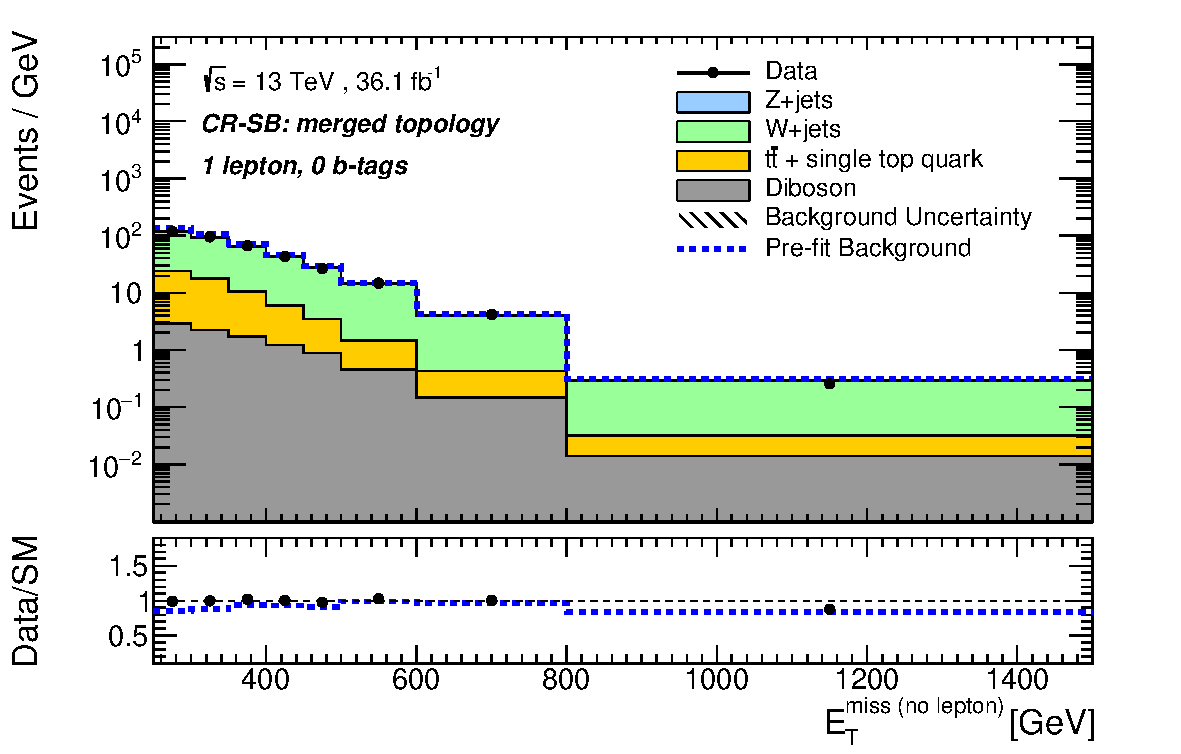
\includegraphics[width=0.95\textwidth]{figures/monoV/postfit/monoV_1lep_0tag_merged_massFail_met_XS.pdf}
    \caption{merged 0 \(b\)-tag}
  \end{subfigure}
    \begin{subfigure}{0.45\textwidth}
    \centering
    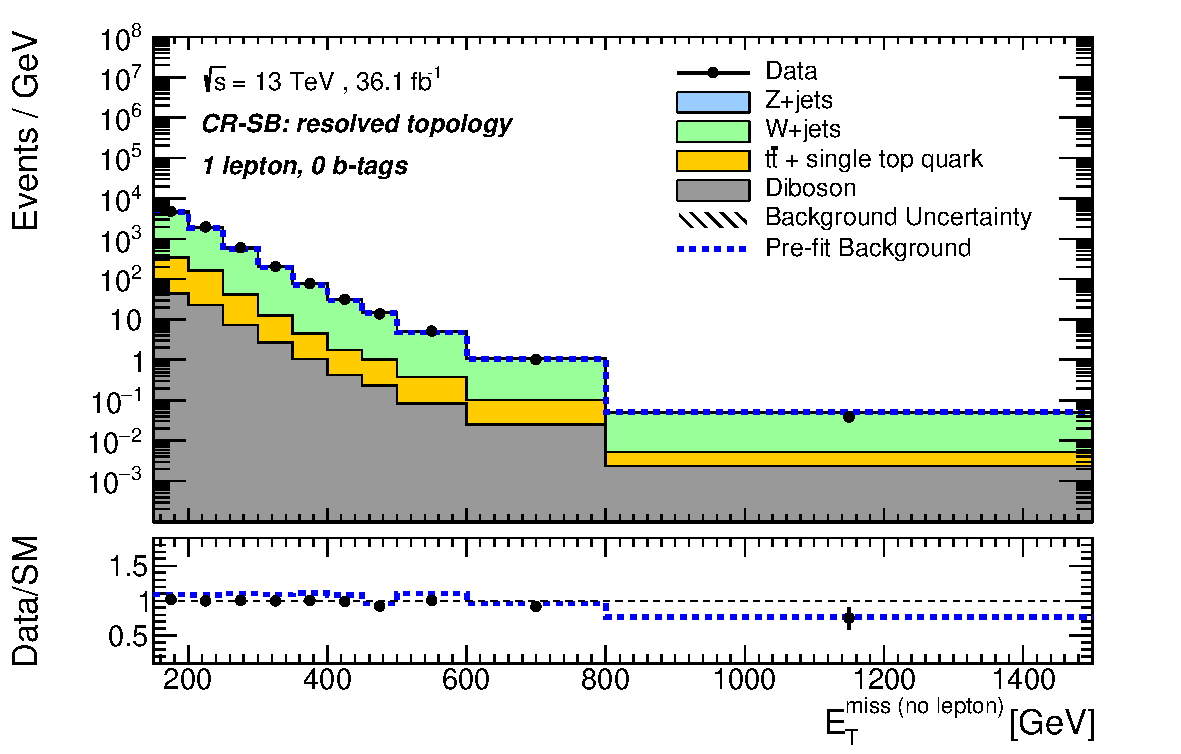
\includegraphics[width=0.95\textwidth]{figures/monoV/postfit/monoV_1lep_0tag_resolved_massFail_met_XS.pdf}
    \caption{resolved 0 \(b\)-tag}
  \end{subfigure} \\

\begin{subfigure}{0.45\textwidth}
    \centering
    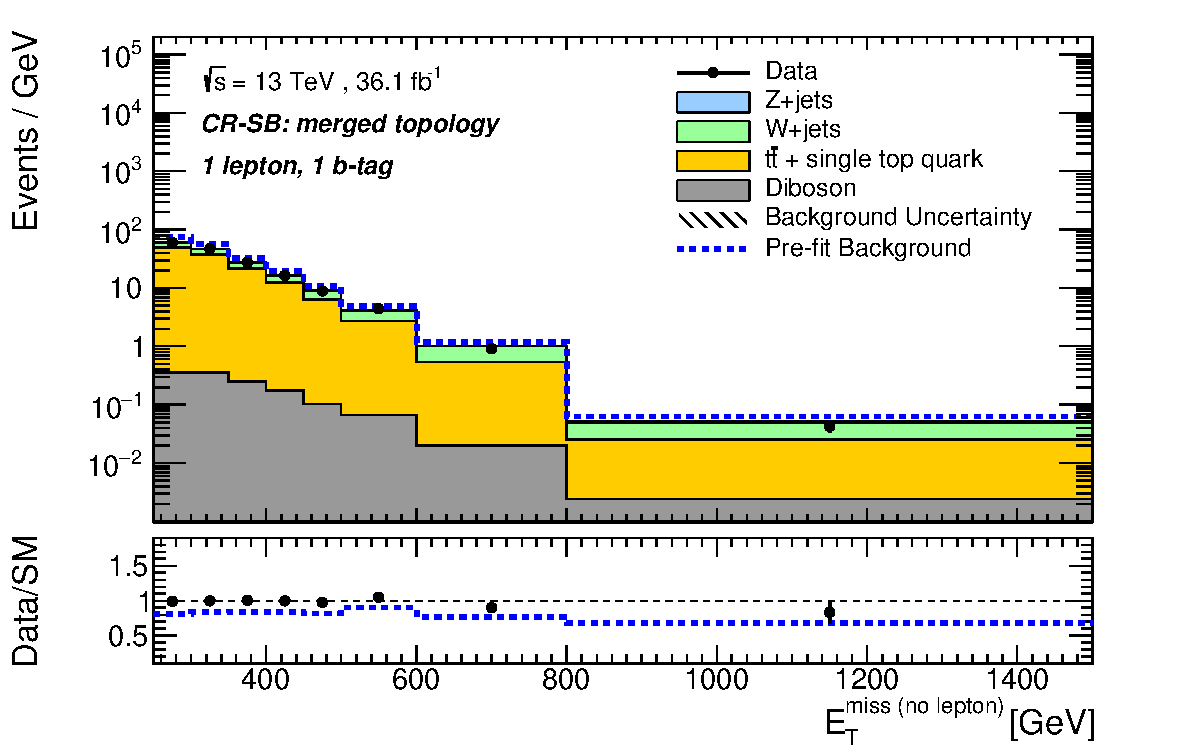
\includegraphics[width=0.95\textwidth]{figures/monoV/postfit/monoV_1lep_1tag_merged_massFail_met_XS.pdf}
    \caption{merged 1 \(b\)-tag}
  \end{subfigure}
    \begin{subfigure}{0.45\textwidth}
    \centering
    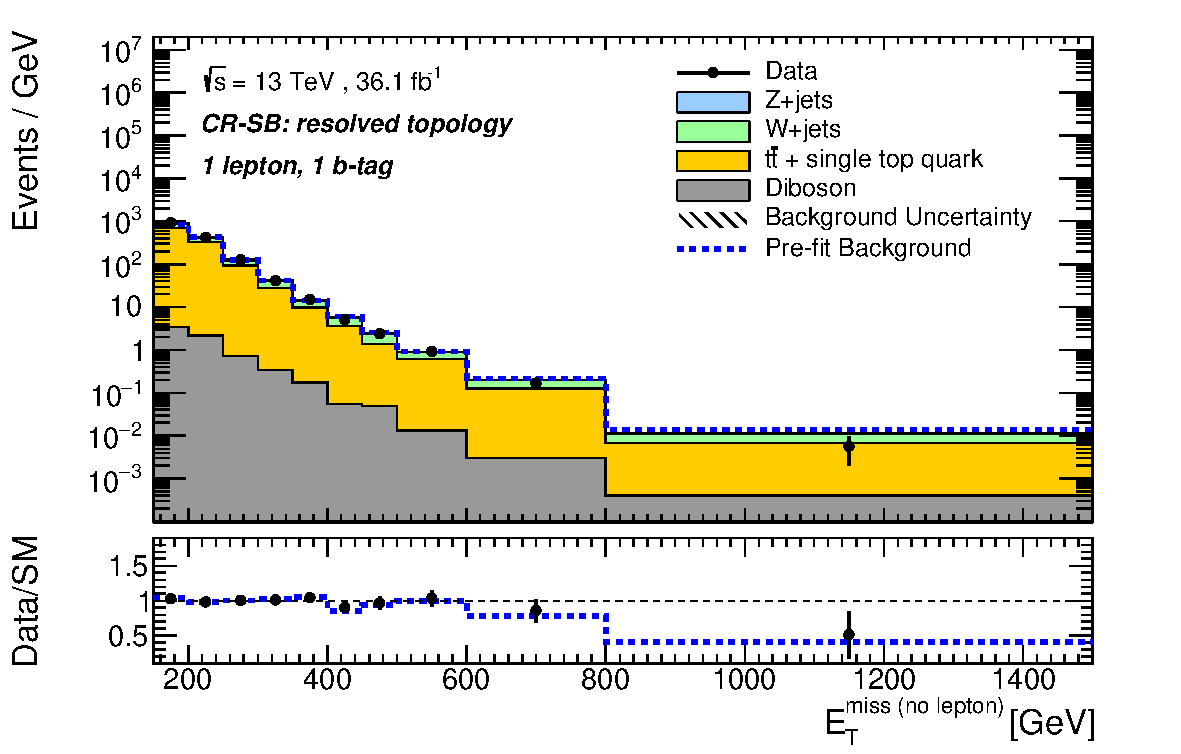
\includegraphics[width=0.95\textwidth]{figures/monoV/postfit/monoV_1lep_1tag_resolved_massFail_met_XS.pdf}
    \caption{resolved 1 \(b\)-tag}
  \end{subfigure} \\

\begin{subfigure}{0.45\textwidth}
    \centering
    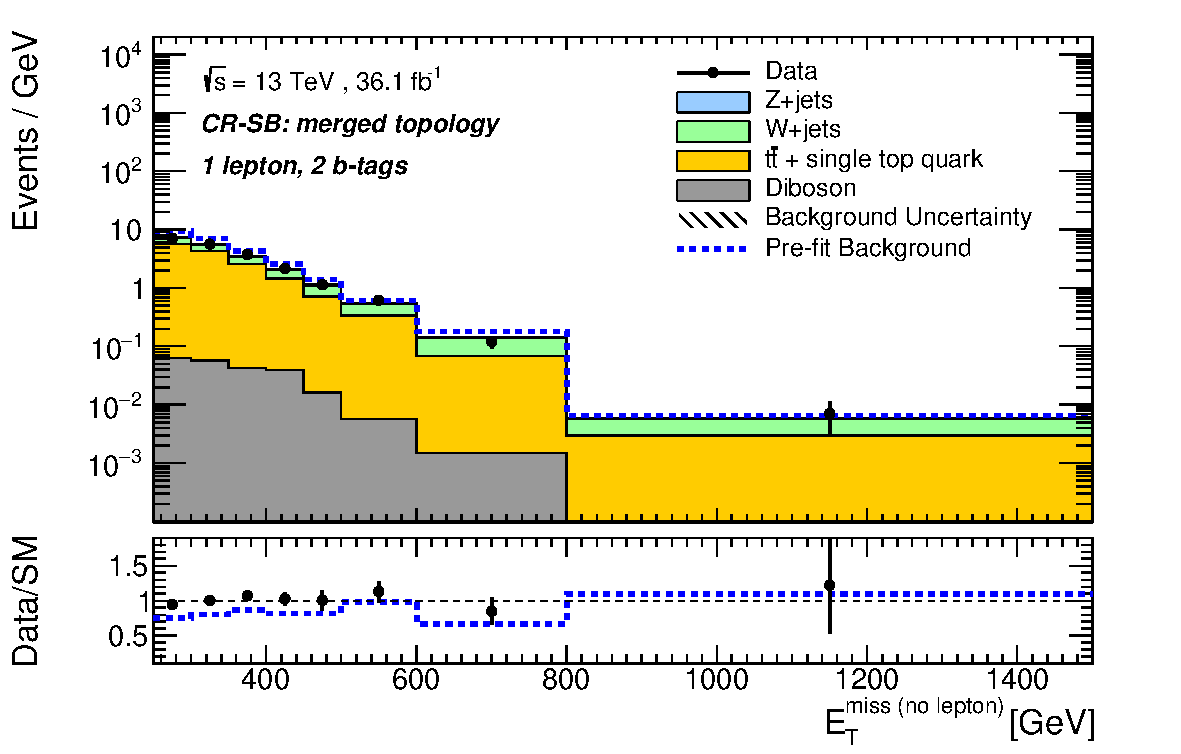
\includegraphics[width=0.95\textwidth]{figures/monoV/postfit/monoV_1lep_2tag_merged_massFail_met_XS.pdf}
    \caption{merged 2 \(b\)-tag}
  \end{subfigure}
    \begin{subfigure}{0.45\textwidth}
    \centering
    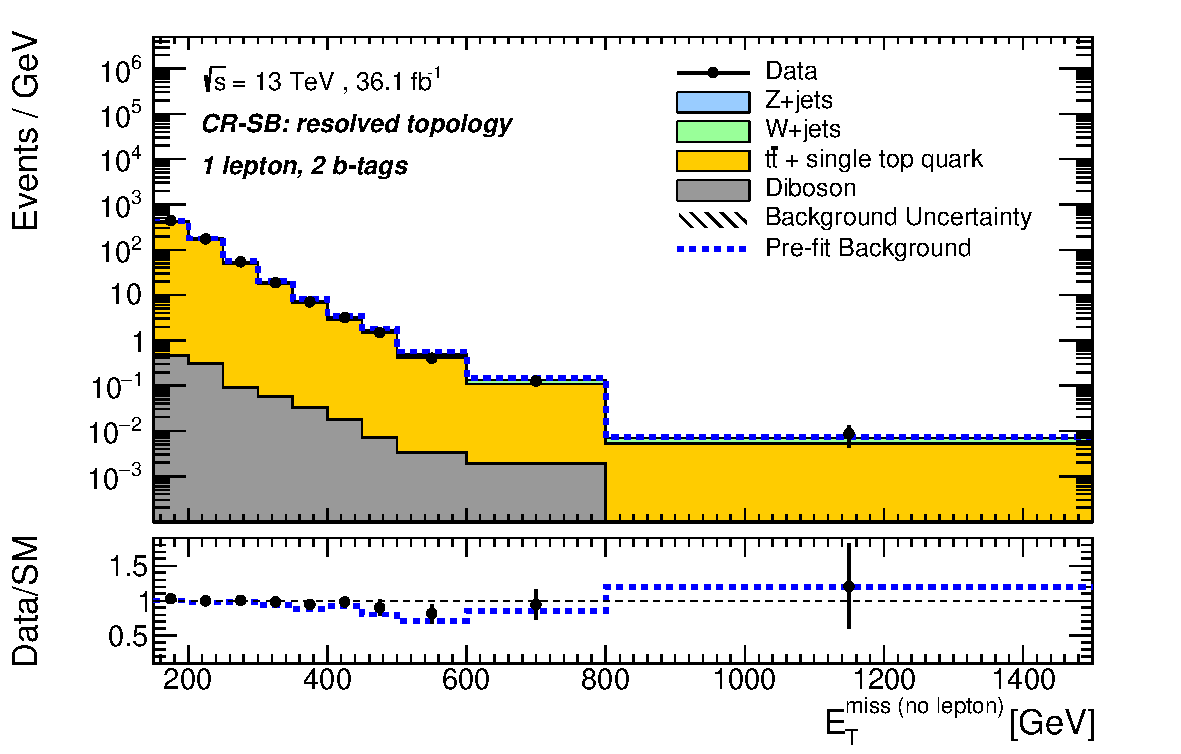
\includegraphics[width=0.95\textwidth]{figures/monoV/postfit/monoV_1lep_2tag_resolved_massFail_met_XS.pdf}
    \caption{resolved 2 \(b\)-tag}
  \end{subfigure}
  \caption{The \metnolep distributions in the 1 muon CR (upper mass side-band) after the background-only fit (\(\mu=0\)) for data (dots) SM background prediction (histograms), shown separately for the merged-topology (left) and resolved-topology (right) event categories with 0 \(b\)-tags (top), 1 \(b\)-tag (middle), and 2 \(b\)-tags (bottom). The total background contribution before the fit to data is shown as a dotted blue line. The hatched area represents the total background uncertainty. The inset at the bottom of each plot shows the ratio of the data to the total post-fit (dots) and pre-fit (dotted blue line) background expectation.}
  \label{fig:appendix:monoV:postfit:cr1}
\end{figure}

\begin{figure}[htbp]
\centering
  \begin{subfigure}{0.45\textwidth}
    \centering
    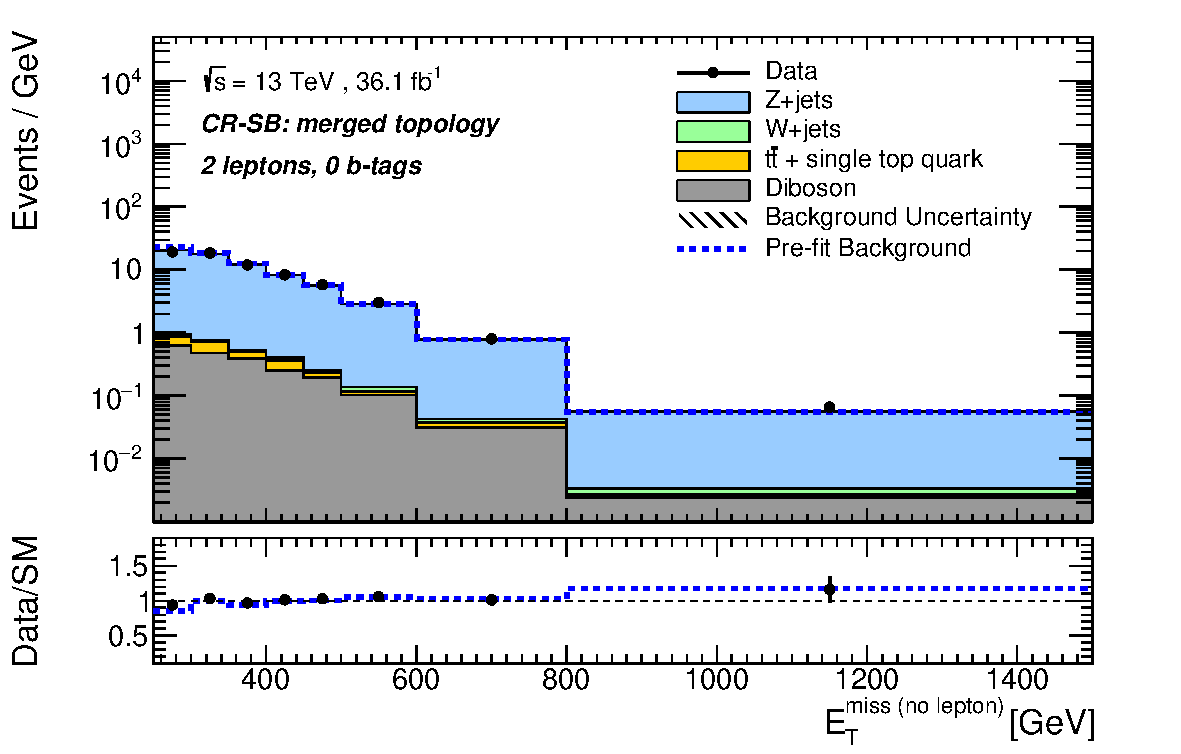
\includegraphics[width=0.95\textwidth]{figures/monoV/postfit/monoV_2lep_0tag_merged_massFail_met_XS.pdf}
    \caption{merged 0 \(b\)-tag}
  \end{subfigure}
    \begin{subfigure}{0.45\textwidth}
    \centering
    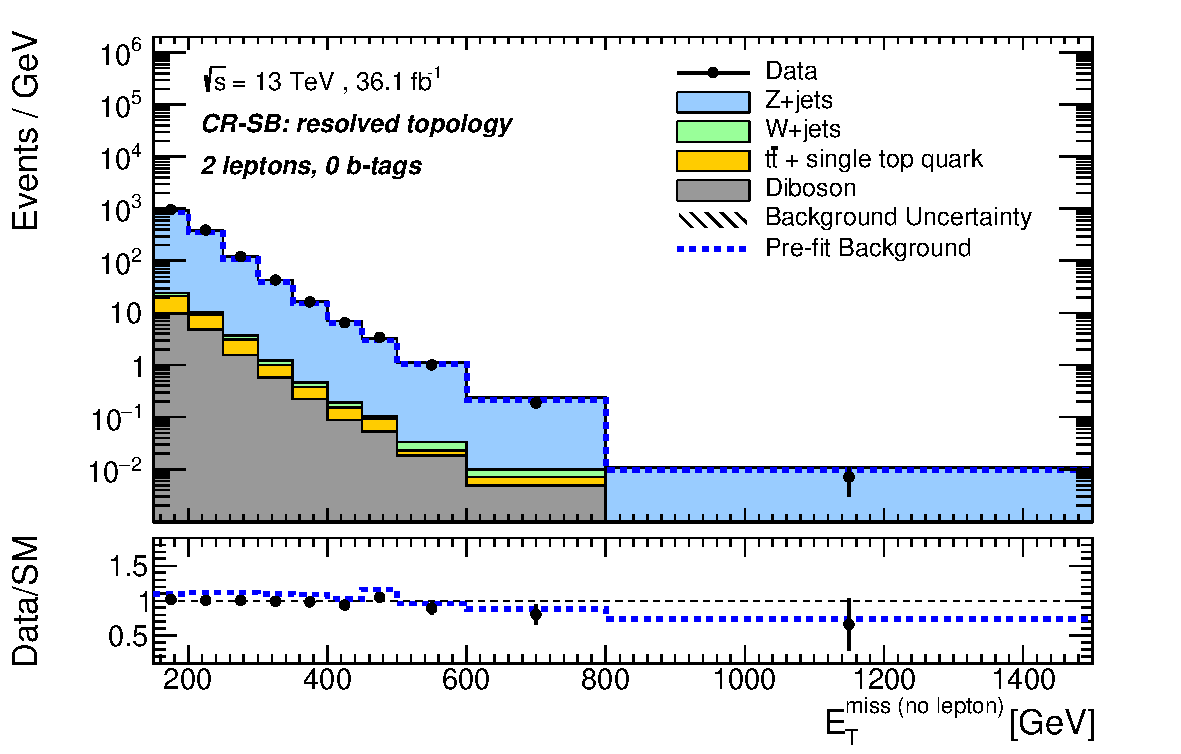
\includegraphics[width=0.95\textwidth]{figures/monoV/postfit/monoV_2lep_0tag_resolved_massFail_met_XS.pdf}
    \caption{resolved 0 \(b\)-tag}
  \end{subfigure} \\

\begin{subfigure}{0.45\textwidth}
    \centering
    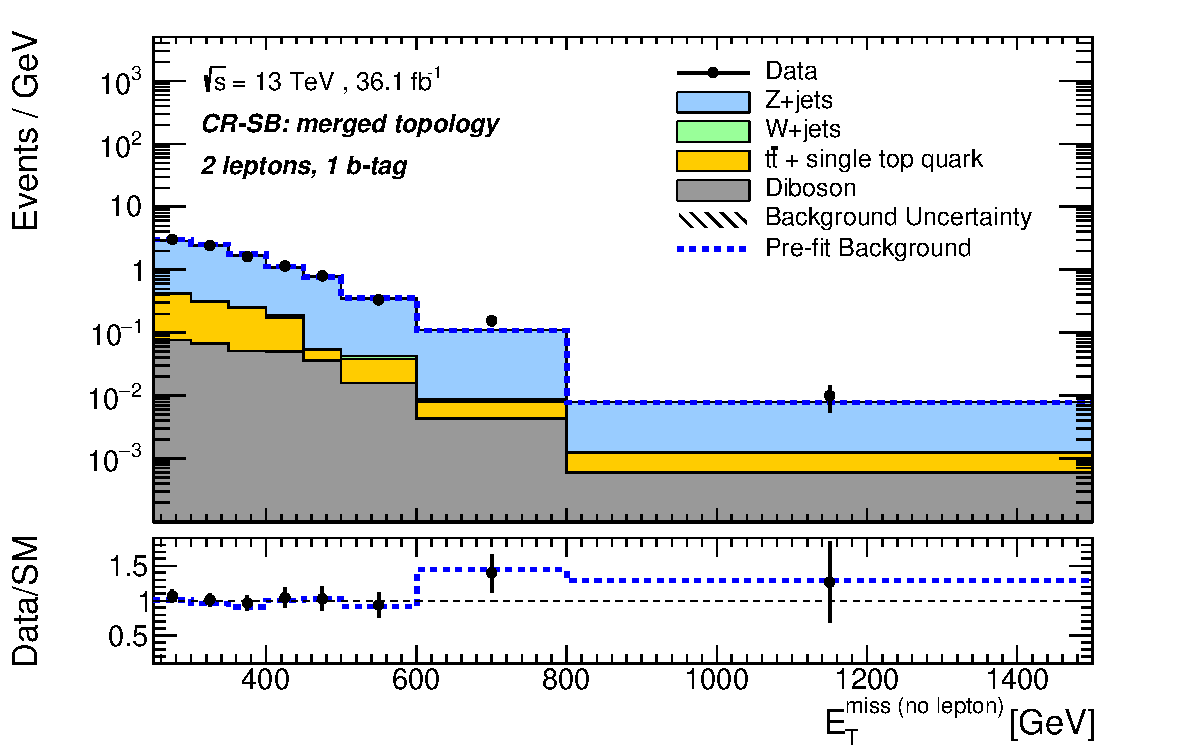
\includegraphics[width=0.95\textwidth]{figures/monoV/postfit/monoV_2lep_1tag_merged_massFail_met_XS.pdf}
    \caption{merged 1 \(b\)-tag}
  \end{subfigure}
    \begin{subfigure}{0.45\textwidth}
    \centering
    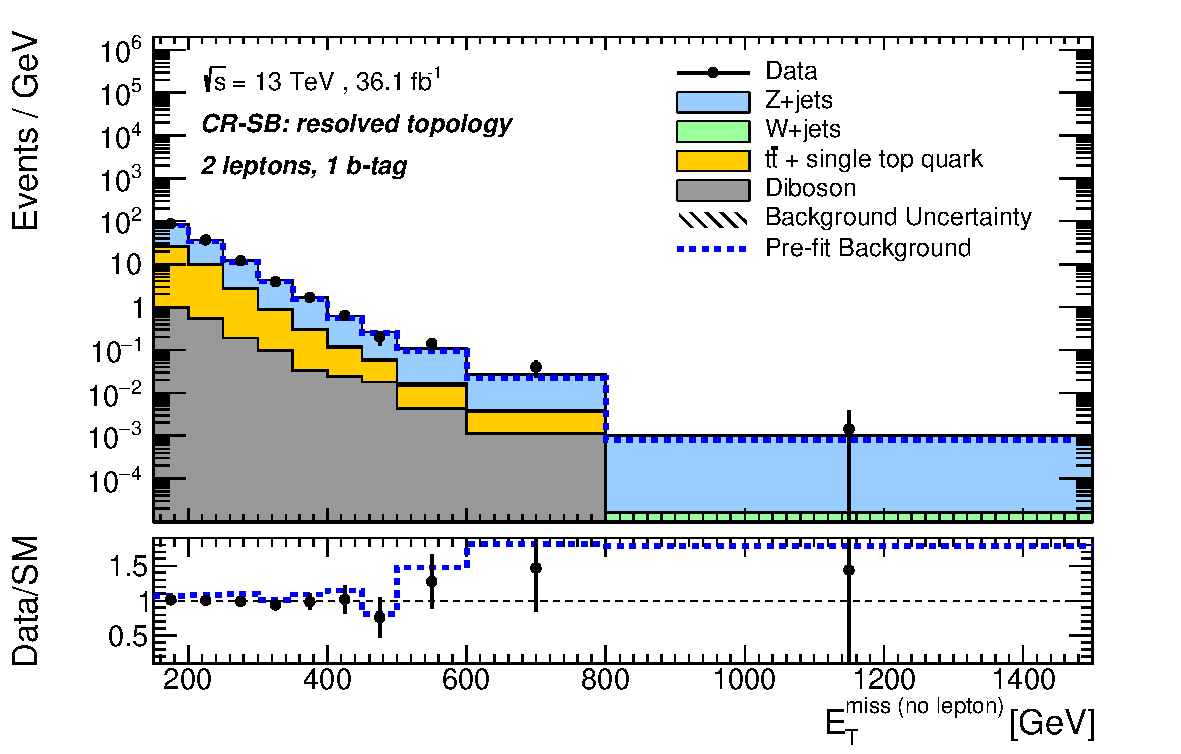
\includegraphics[width=0.95\textwidth]{figures/monoV/postfit/monoV_2lep_1tag_resolved_massFail_met_XS.pdf}
    \caption{resolved 1 \(b\)-tag}
  \end{subfigure} \\

\begin{subfigure}{0.45\textwidth}
    \centering
    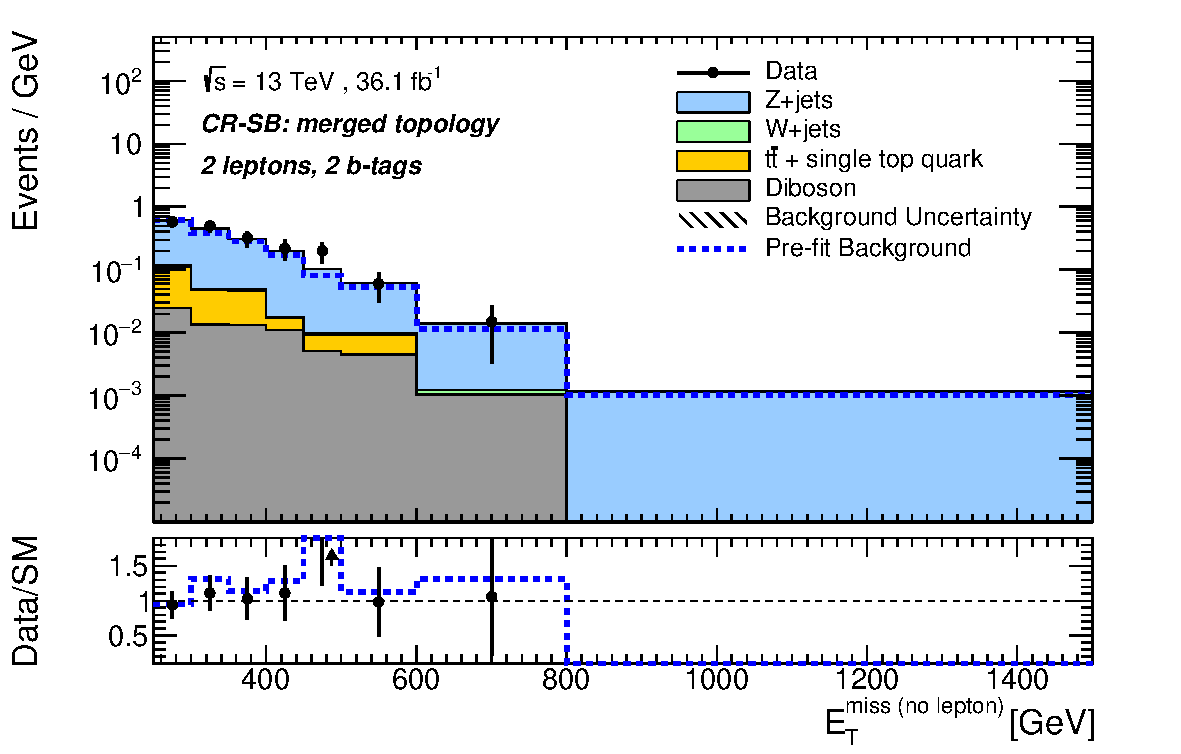
\includegraphics[width=0.95\textwidth]{figures/monoV/postfit/monoV_2lep_2tag_merged_massFail_met_XS.pdf}
    \caption{merged 2 \(b\)-tag}
  \end{subfigure}
    \begin{subfigure}{0.45\textwidth}
    \centering
    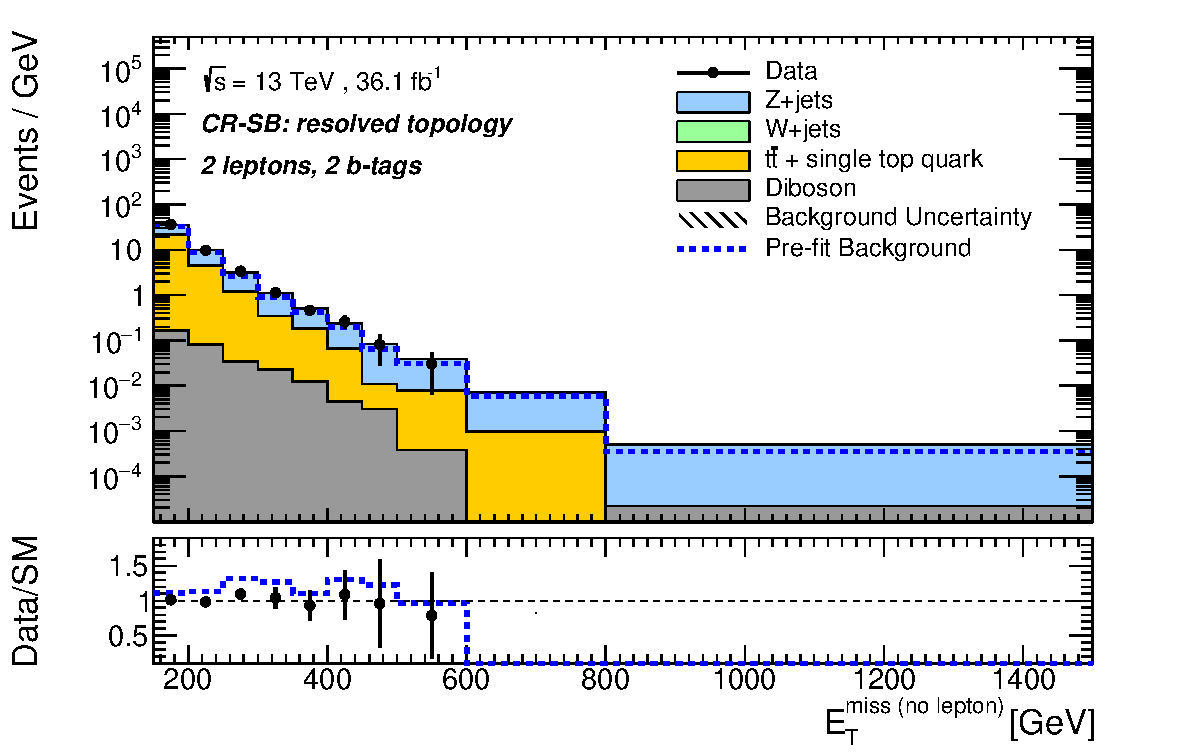
\includegraphics[width=0.95\textwidth]{figures/monoV/postfit/monoV_2lep_2tag_resolved_massFail_met_XS.pdf}
    \caption{resolved 2 \(b\)-tag}
  \end{subfigure}
  \caption{The \metnolep distributions in the 2 lepton CR (upper mass side-band) after the background-only fit (\(\mu=0\)) for data (dots) SM background prediction (histograms), shown separately for the merged-topology (left) and resolved-topology (right) event categories with 0 \(b\)-tags (top), 1 \(b\)-tag (middle), and 2 \(b\)-tags (bottom). The total background contribution before the fit to data is shown as a dotted blue line. The hatched area represents the total background uncertainty. The inset at the bottom of each plot shows the ratio of the data to the total post-fit (dots) and pre-fit (dotted blue line) background expectation.}
  \label{fig:appendix:monoV:postfit:cr2}
\end{figure}



\section{Triggers used in the \(\met + V(\Pq\Pq)\) search}
\label{sec:appendix:monoV:trigger}

A summary of all triggers employed in the \(\met + \HepProcess{V(\Pq\Pq)}\) search is provided in \Cref{tab:appendix:monoV:trigger:summary}.

\begin{table}[htbp]
\caption{List of triggers applied in the \(\met + \HepProcess{V(\Pq\Pq)}\) search using data recorded during 2015--2016 data taking.}
\label{tab:appendix:monoV:trigger:summary}
\resizebox{1.\textwidth}{!}{%
\begin{tabular}{l l l}
\toprule
period & 0 + 1 lepton & 2 lepton \\
\midrule
\multirow{6}{*}{2015} & \multirow{6}{*}{\textsc{HLT\_xe70}} & \textsc{HLT\_e24\_lhmedium\_L1EM18VH} (MC) \\
& & \textsc{HLT\_e24\_lhmedium\_L1EM20VH} (data) \\
& & \textbf{OR} \textsc{HLT\_e60\_lhmedium} \\
& & \textbf{OR} \textsc{HLT\_e120\_lhloose}  \\
& & \textbf{OR} \textsc{HLT\_mu20\_iloose\_L1MU15} \\
& & \textbf{OR} \textsc{HLT\_mu50} \\
\midrule
\multirow{8}{*}{2016 (A)} & \multirow{8}{*}{\textsc{HLT\_xe90\_mht\_L1XE50}} & \textsc{HLT\_e24\_lhtight\_nod0\_ivarloose} \\
& & \textbf{OR} \textsc{HLT\_e60\_lhmedium\_nod0} \\
& & \textbf{OR} \textsc{HLT\_e60\_medium} \\
& & \textbf{OR} \textsc{HLT\_e140\_lhloose\_nod0} \\
& & \textbf{OR} \textsc{HLT\_e300\_etcut} \\
& & \textbf{OR} \textsc{HLT\_mu24\_iloose\_L1MU15} (MC) \\
& & \textbf{OR} \textsc{HLT\_mu24\_iloose} (data) \\
& & \textbf{OR} \textsc{HLT\_mu40} \\
\midrule
\multirow{3}{*}{2016 (B--D3)} & \multirow{3}{*}{\textsc{HLT\_xe90\_mht\_L1XE50}} & \textsc{HLT\_e24\_lhtight\_nod0\_ivarloose} \\
& & \textbf{OR} \textsc{HLT\_mu24\_imedium} (data) \\
& & \textbf{OR} \textsc{HLT\_mu50} \\
\midrule
\multirow{2}{*}{2016 (D4--E3)} & \textsc{HLT\_xe100\_mht\_L1XE50} & \textsc{HLT\_e26\_lhtight\_nod0\_ivarloose} \\
& \textbf{OR} \textsc{HLT\_xe110\_mht\_L1XE50} & \textbf{OR} \textsc{HLT\_mu24\_ivarmedium} (data) \\
\midrule
\multirow{7}{*}{2016 (F--L)} & \multirow{7}{*}{\textsc{HLT\_xe110\_mht\_L1XE50}} & \textsc{HLT\_e26\_lhtight\_nod0\_ivarloose} \\
& & \textbf{OR} \textsc{HLT\_e60\_lhmedium\_nod0} \\
& & \textbf{OR} \textsc{HLT\_e60\_medium} \\
& & \textbf{OR} \textsc{HLT\_e140\_lhloose\_nod0} \\
& & \textbf{OR} \textsc{HLT\_e300\_etcut} \\
& & \textbf{OR} \textsc{HLT\_mu24\_ivarmedium} \\
& & \textbf{OR} \textsc{HLT\_mu50} \\
\bottomrule
\end{tabular}%
}
\end{table}

Collision events with \met as low as \SI{150}{\giga\electronvolt} are considered in the \(\met + \HepProcess{V(\Pq\Pq)}\) search. Because the \met trigger is not fully efficient in this range, the trigger efficiency is measured in events and correction factors are applied to the simulated samples in order to match the efficiencies measured in data.

The procedure for calculating the \met trigger correction factors is described in \Cref{sec:common:data:trigger}.
The events selected for the \met trigger calibration are selected by the single-muon triggers listed in \Cref{tab:appendix:monoV:trigger:summary} and are required to contain no baseline electrons and exactly one signal or tight signal muon. The selection requirements are similar to that of the resolved signal region (introduced in \Cref{sec:monoV:selection}) except for the \metnolep and \mptnolep cuts, which are dropped from the selection requirements.

\Cref{fig:appendix:monoV:trigger:mettriggerefficiency} shows the \met trigger scale-factors for the \(\met + V(\Pq\Pq)\) search search obtained from the selection inclusive in \bjets compared to the \met trigger scale-factors obtained from the selection requiring at least one \btagged jet.

\begin{figure}[htbp]
  \centering
  \begin{subfigure}{0.49\textwidth}
    \centering
    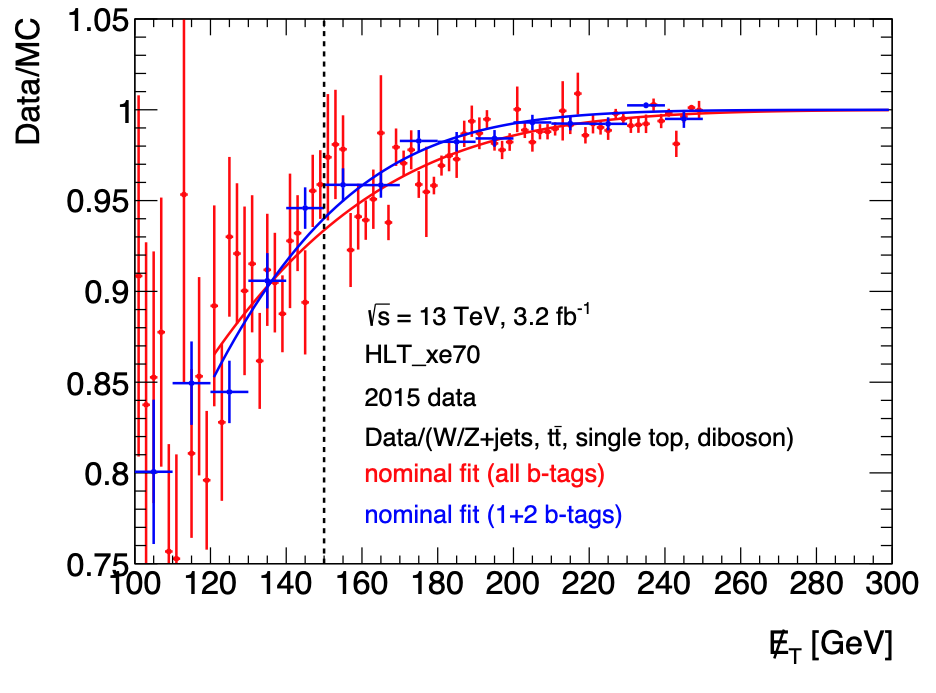
\includegraphics[width=1.\textwidth]{figures/monoV/monoVtriggersf_HLTxe70.png}
    \caption{\textsc{HLT\_xe70} \met trigger}
  \end{subfigure}
    \begin{subfigure}{0.49\textwidth}
    \centering
    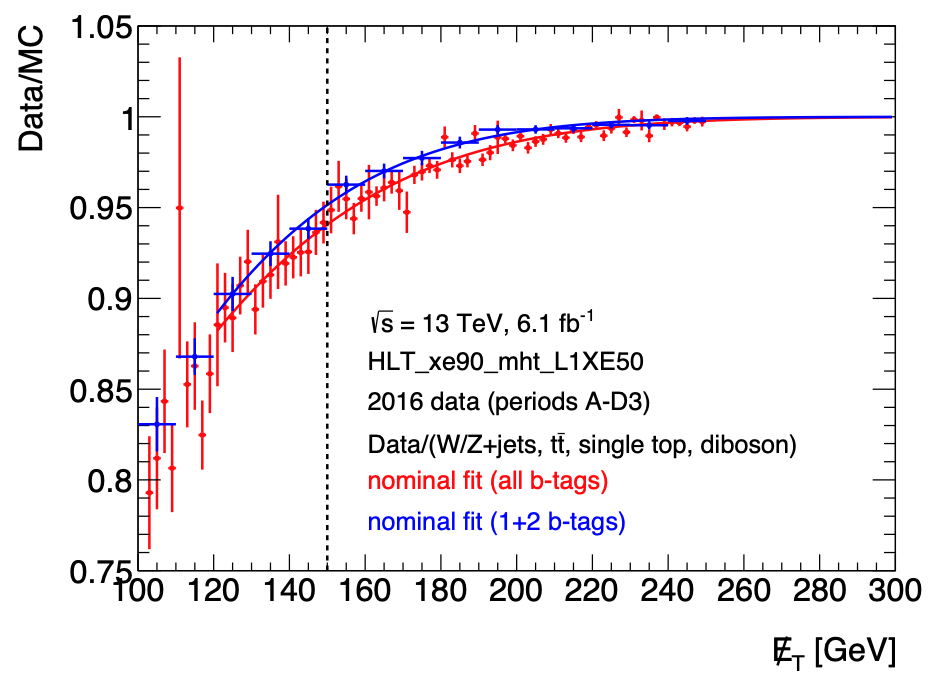
\includegraphics[width=1.\textwidth]{figures/monoV/monoVtriggersf_HLTxe90.png}
    \caption{\textsc{HLT\_xe90\_mht\_L1XE50} \met trigger}
  \end{subfigure}
  \\
  \begin{subfigure}{0.49\textwidth}
    \centering
    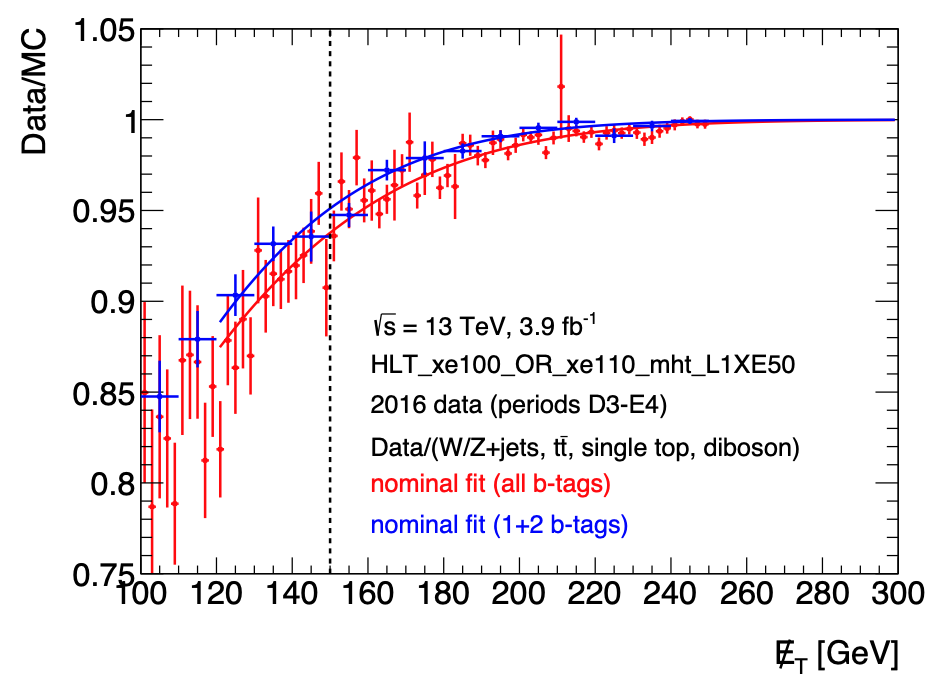
\includegraphics[width=1.\textwidth]{figures/monoV/monoVtriggersf_HLTxe100.png}
    \caption{\textsc{HLT\_xe100\_mht\_L1XE50} \met trigger}
  \end{subfigure}
    \begin{subfigure}{0.49\textwidth}
    \centering
    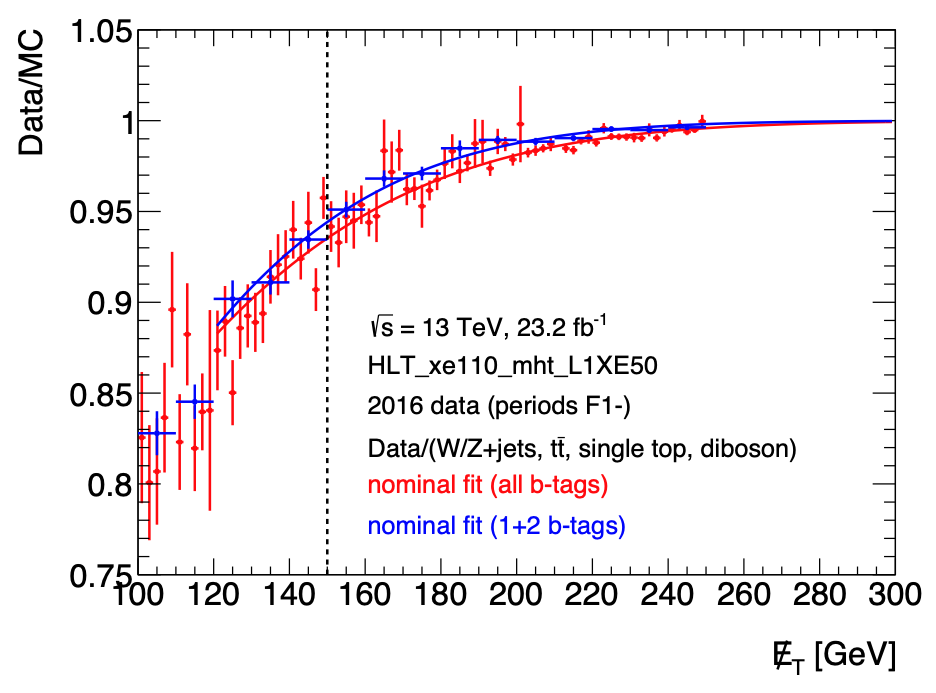
\includegraphics[width=1.\textwidth]{figures/monoV/monoVtriggersf_HLTxe110.png}
    \caption{\textsc{HLT\_xe110\_mht\_L1XE50} \met trigger}
  \end{subfigure}
  \caption{\met trigger scale-factors as a function of \met obtained from a selection inclusive in \bjets (red) and from a selection requiring at least one \(b\)-jet (blue) for the \met triggers \textsc{HLT\_xe70}, \textsc{HLT\_xe90\_mht\_L1XE50}, \textsc{HLT\_xe100\_mht\_L1XE50}, and \textsc{HLT\_xe110\_mht\_L1XE50}.}
  \label{fig:appendix:monoV:trigger:mettriggerefficiency}
\end{figure}


\section{Triggers used in the \(\met + \PHiggs(\Pqb\Paqb)\) search}
\label{sec:appendix:monoH:trigger}

A summary of all triggers employed in the \(\met + \HepProcess{\PHiggs(\Pqb\Paqb)}\) search is provided in \Cref{tab:appendix:monoH:trigger:summary}.

\begin{table}[hbtp]
\caption{List of triggers applied in the \(\met + \HepProcess{\PHiggs(\Pqb\Paqb)}\) search using data recorded during 2015--2017 data taking.}
\label{tab:appendix:monoH:trigger:summary}
\resizebox{1.\textwidth}{!}{%
\begin{tabular}{l l l}
\toprule
period & 0 + 1 lepton & 2 lepton \\
\midrule
\multirow{6}{*}{2015} & \multirow{6}{*}{\textsc{HLT\_xe70}} & \textsc{HLT\_e24\_lhmedium\_L1EM18VH} (MC) \\
& & \textsc{HLT\_e24\_lhmedium\_L1EM20VH} (data) \\
& & \textbf{OR} \textsc{HLT\_e60\_lhmedium} \\
& & \textbf{OR} \textsc{HLT\_e120\_lhloose}  \\
& & \textbf{OR} \textsc{HLT\_mu20\_iloose\_L1MU15} \\
& & \textbf{OR} \textsc{HLT\_mu50} \\
\midrule
\multirow{8}{*}{2016 (A)} & \multirow{8}{*}{\textsc{HLT\_xe90\_mht\_L1XE50}} & \textsc{HLT\_e24\_lhtight\_nod0\_ivarloose} \\
& & \textbf{OR} \textsc{HLT\_e60\_lhmedium\_nod0} \\
& & \textbf{OR} \textsc{HLT\_e60\_medium} \\
& & \textbf{OR} \textsc{HLT\_e140\_lhloose\_nod0} \\
& & \textbf{OR} \textsc{HLT\_e300\_etcut} \\
& & \textbf{OR} \textsc{HLT\_mu24\_iloose\_L1MU15} (MC) \\
& & \textbf{OR} \textsc{HLT\_mu24\_iloose} (data) \\
& & \textbf{OR} \textsc{HLT\_mu40} \\
\midrule
\multirow{3}{*}{2016 (B--D3)} & \multirow{3}{*}{\textsc{HLT\_xe90\_mht\_L1XE50}} & \textsc{HLT\_e24\_lhtight\_nod0\_ivarloose} \\
& & \textbf{OR} \textsc{HLT\_mu24\_imedium} (data) \\
& & \textbf{OR} \textsc{HLT\_mu50} \\
\midrule
\multirow{2}{*}{2016 (D4--E3)} & \textsc{HLT\_xe100\_mht\_L1XE50} & \textsc{HLT\_e26\_lhtight\_nod0\_ivarloose} \\
& \textbf{OR} \textsc{HLT\_xe110\_mht\_L1XE50} & \textbf{OR} \textsc{HLT\_mu24\_ivarmedium} (data) \\
\midrule
\multirow{7}{*}{2016 (F--L)} & \multirow{7}{*}{\textsc{HLT\_xe110\_mht\_L1XE50}} & \textsc{HLT\_e26\_lhtight\_nod0\_ivarloose} \\
& & \textbf{OR} \textsc{HLT\_e60\_lhmedium\_nod0} \\
& & \textbf{OR} \textsc{HLT\_e60\_medium} \\
& & \textbf{OR} \textsc{HLT\_e140\_lhloose\_nod0} \\
& & \textbf{OR} \textsc{HLT\_e300\_etcut} \\
& & \textbf{OR} \textsc{HLT\_mu24\_ivarmedium} \\
& & \textbf{OR} \textsc{HLT\_mu50} \\
\midrule
\multirow{7}{*}{2017} & \multirow{7}{*}{\textsc{HLT\_xe110\_pufit\_L1XE55}} & \textsc{HLT\_e26\_lhtight\_nod0\_ivarloose} \\
& & \textbf{OR} \textsc{HLT\_e60\_lhmedium\_nod0} \\
& & \textbf{OR} \textsc{HLT\_e140\_lhloose\_nod0} \\
& & \textbf{OR} \textsc{HLT\_e300\_etcut} \\
& & \textbf{OR} \textsc{HLT\_mu26\_ivarmedium} \\
& & \textbf{OR} \textsc{HLT\_mu50} \\
& & \textbf{OR} \textsc{HLT\_mu60\_0eta105\_msonly} \\
\bottomrule
\end{tabular}%
}
\end{table}

Collision events with \met as low as \SI{150}{\giga\electronvolt} are considered in the \(\met + \HepProcess{\PHiggs(\Pqb\Paqb)}\) search. Because the \met trigger is not fully efficient in this range, the trigger efficiency is measured in events and correction factors are applied to the simulated samples in order to match the efficiencies measured in data.

The procedure for calculating the \met trigger correction factors is described in \Cref{sec:common:data:trigger}.
The \MET trigger efficiency is estimated with an event selection almost identical to the signal region (c.f. \Cref{sec:monoH:selection}, with the exceptions that
\begin{itemize}
  \item single muon triggers and a requirement of exactly one muon in the event are used,
  \item the selection requirement on the \met significance is based on \metnomu, and
  \item the requirements on \met and \mpt are dropped.
\end{itemize}

\Cref{fig:appendix:monoH:trigger:mettriggerefficiency} shows the \met trigger scale-factors obtained from the selection inclusive in \bjets compared to the \met trigger scale-factors obtained from the selection requiring at least one \btagged jet.

\begin{figure}[htbp]
  \centering
  \begin{subfigure}{0.45\textwidth}
    \centering
    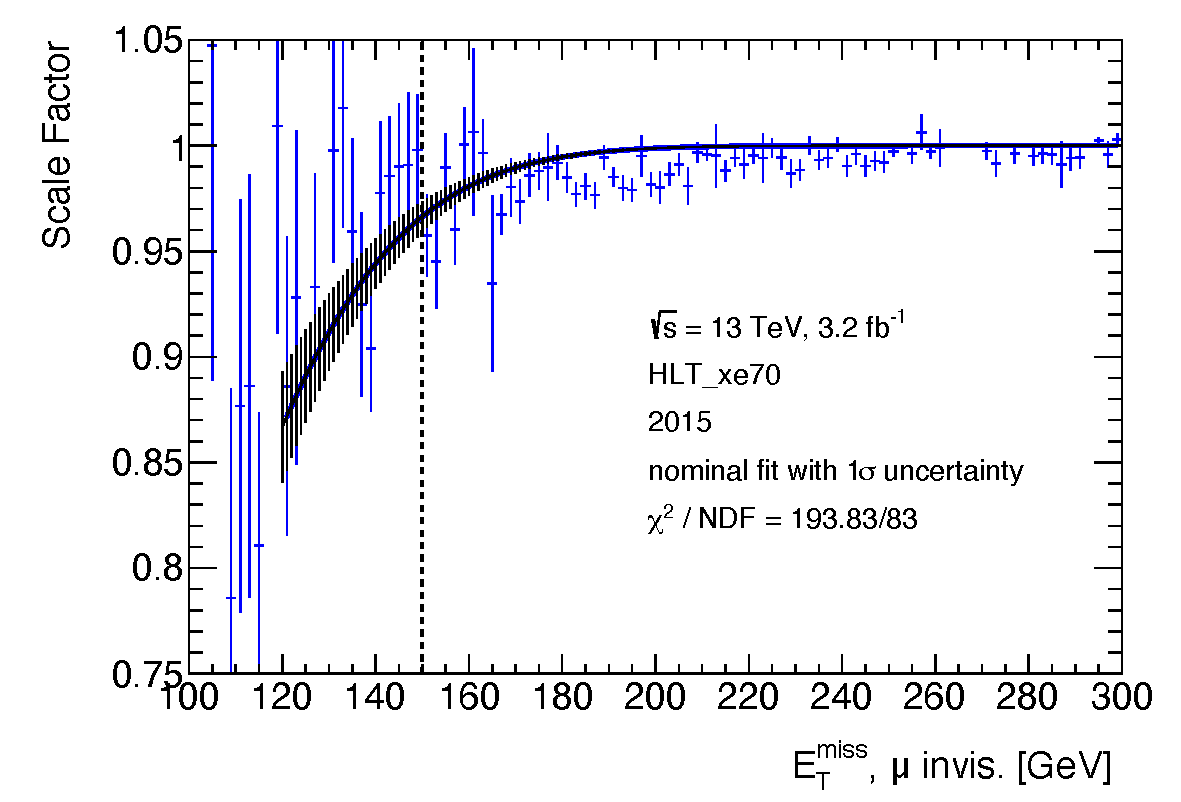
\includegraphics[width=0.95\textwidth]{figures/monoH/trigger/figures_TriggerScaleFactors_SF_HLT_xe70.pdf}
    \caption{\textsc{HLT\_xe70} \met trigger}
  \end{subfigure}
    \begin{subfigure}{0.45\textwidth}
    \centering
    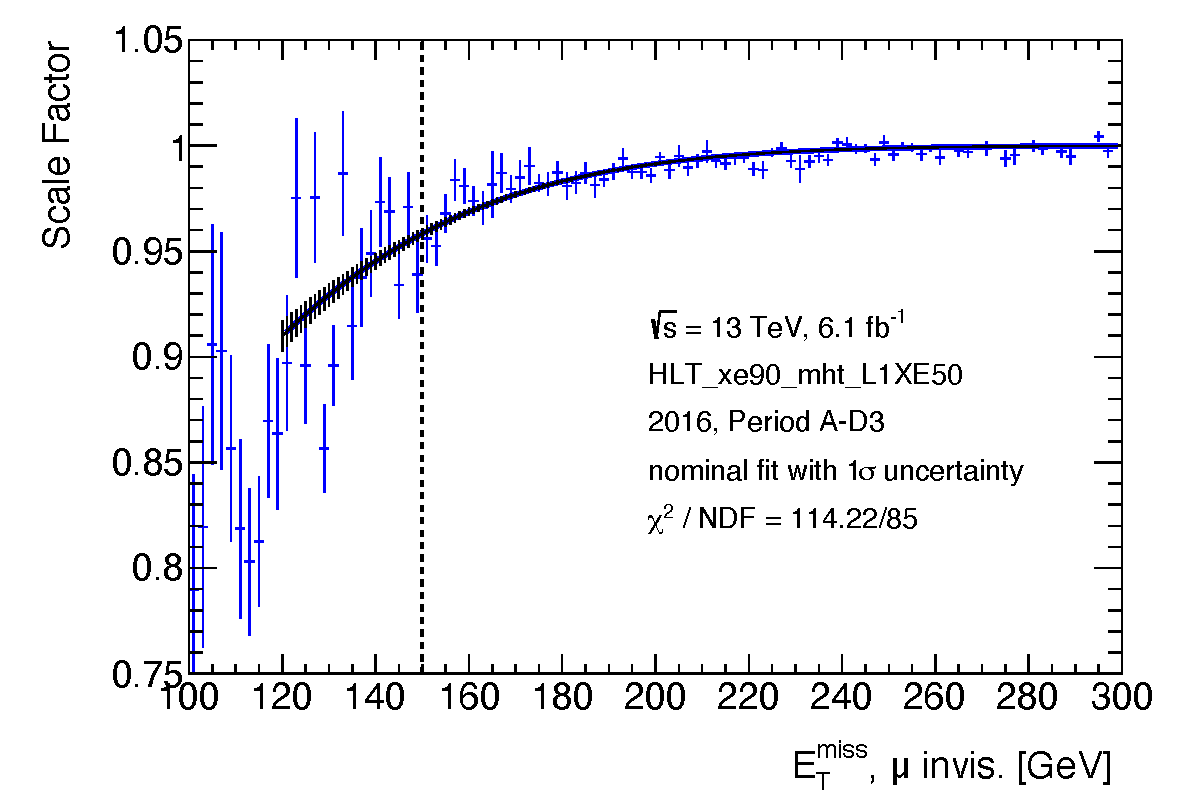
\includegraphics[width=0.95\textwidth]{figures/monoH/trigger/figures_TriggerScaleFactors_SF_HLT_xe90_mht_L1XE50.pdf}
    \caption{\textsc{HLT\_xe90\_mht\_L1XE50} \met trigger}
  \end{subfigure}
  \\
  \begin{subfigure}{0.45\textwidth}
    \centering
    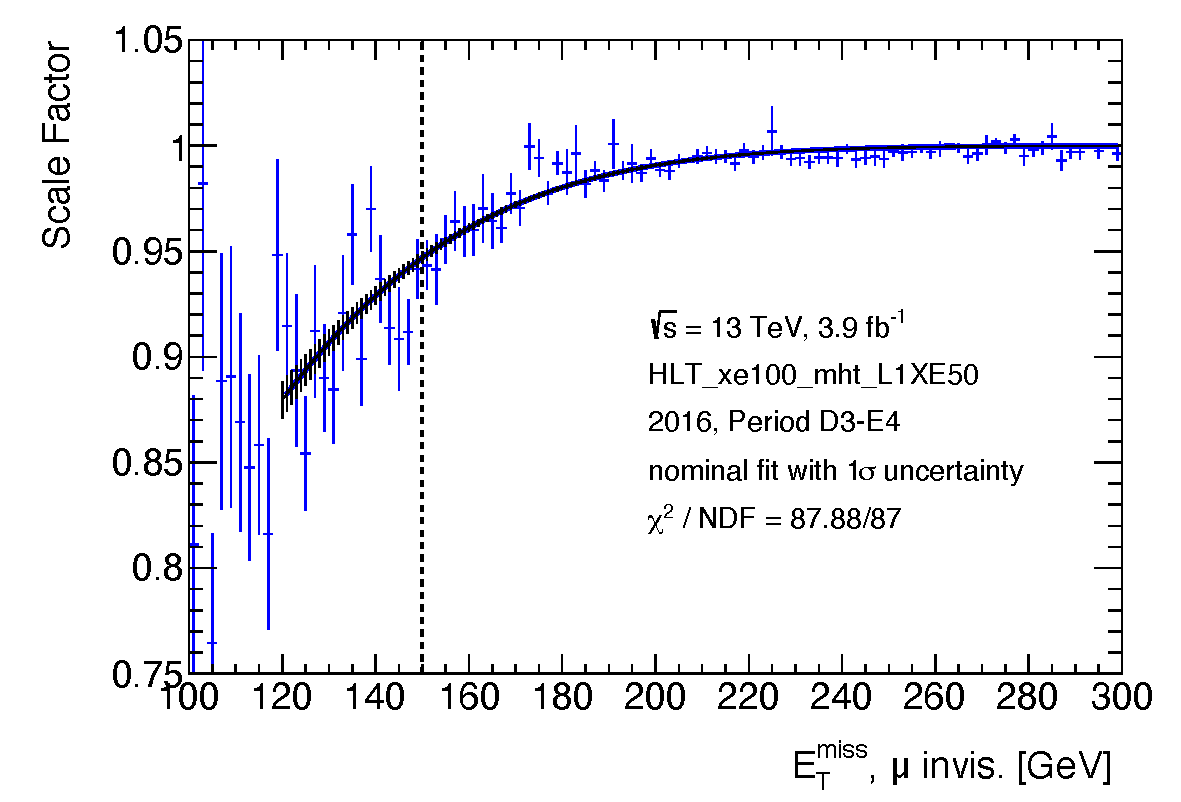
\includegraphics[width=0.95\textwidth]{figures/monoH/trigger/figures_TriggerScaleFactors_SF_HLT_xe100_mht_L1XE50.pdf}
    \caption{\textsc{HLT\_xe100\_mht\_L1XE50} \met trigger}
  \end{subfigure}
    \begin{subfigure}{0.45\textwidth}
    \centering
    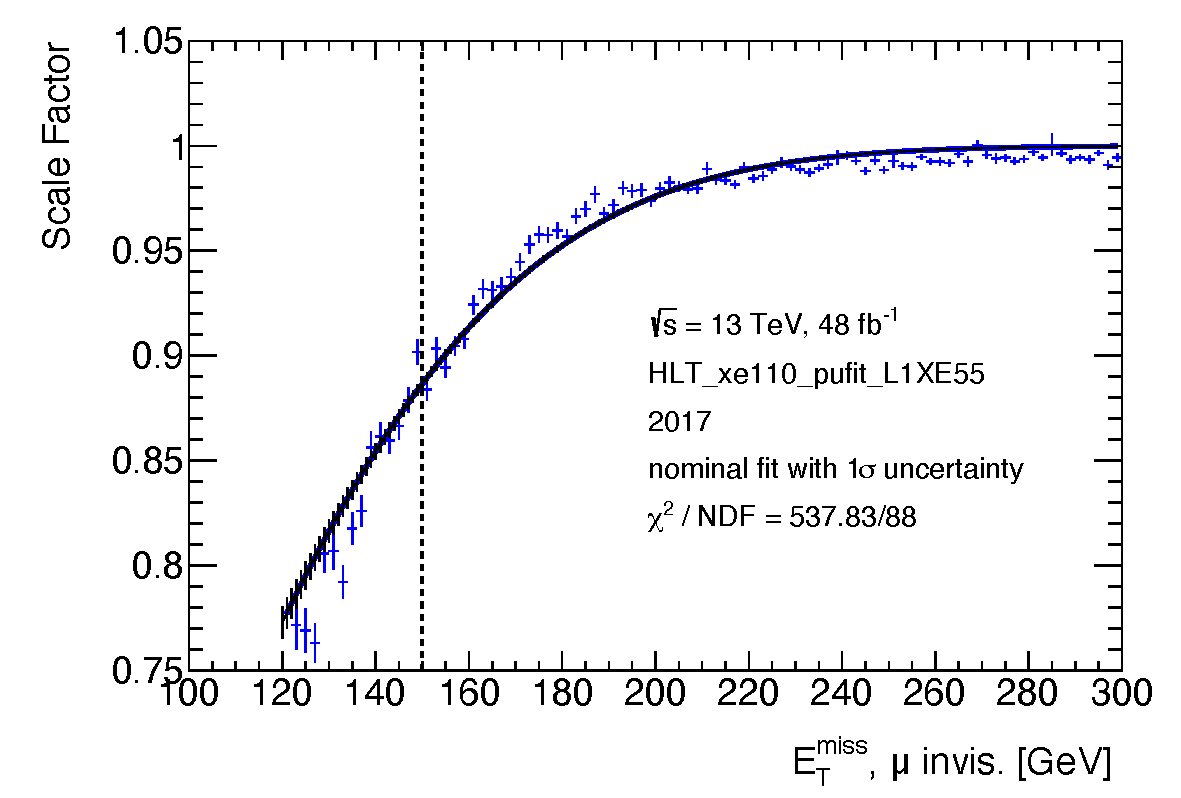
\includegraphics[width=0.95\textwidth]{figures/monoH/trigger/figures_TriggerScaleFactors_SF_HLT_xe110_pufit_L1XE55.pdf}
    \caption{\textsc{HLT\_xe110\_pufit\_L1XE55} \met trigger}
  \end{subfigure}
  \caption{\met trigger scale-factors as a function of \met obtained from a selection inclusive in \bjets for the \met triggers \textsc{HLT\_xe70}, \textsc{HLT\_xe90\_mht\_L1XE50}, \textsc{HLT\_xe100\_mht\_L1XE50}, and \textsc{HLT\_xe110\_pufit\_L1XE55}. The hatched band shows the \(\pm 1 \sigma\) fit uncertainty}
  \label{fig:appendix:monoH:trigger:mettriggerefficiency}
\end{figure}


\section{Triggers used in the \(\met + s(VV)\) hadronic search}
\label{sec:appendix:monoS:trigger}

A summary of all triggers employed in the \(\met + \HepProcess{s(VV)}\) hadronic search is provided in \Cref{tab:appendix:monoS:trigger:summary}.

\begin{table}[hbtp]
\caption{List of triggers applied in the \(\met + \HepProcess{\HepProcess{s(VV)}}\) hadronic search using data recorded during 2015--2018 data taking.}
\label{tab:appendix:monoS:trigger:summary}
\footnotesize{
\centering
\resizebox{.6\textwidth}{!}{
\begin{tabular}{l l l}
\toprule
period & 0 + 1 lepton & 2 lepton \\
\midrule
\multirow{6}{*}{2015} & \multirow{6}{*}{\textsc{HLT\_xe70}} & \textsc{HLT\_e24\_lhmedium\_L1EM18VH} (MC) \\
& & \textsc{HLT\_e24\_lhmedium\_L1EM20VH} (data) \\
& & \textbf{OR} \textsc{HLT\_e60\_lhmedium} \\
& & \textbf{OR} \textsc{HLT\_e120\_lhloose}  \\
& & \textbf{OR} \textsc{HLT\_mu20\_iloose\_L1MU15} \\
& & \textbf{OR} \textsc{HLT\_mu50} \\
\midrule
\multirow{8}{*}{2016 (A)} & \multirow{8}{*}{\textsc{HLT\_xe90\_mht\_L1XE50}} & \textsc{HLT\_e24\_lhtight\_nod0\_ivarloose} \\
& & \textbf{OR} \textsc{HLT\_e60\_lhmedium\_nod0} \\
& & \textbf{OR} \textsc{HLT\_e60\_medium} \\
& & \textbf{OR} \textsc{HLT\_e140\_lhloose\_nod0} \\
& & \textbf{OR} \textsc{HLT\_e300\_etcut} \\
& & \textbf{OR} \textsc{HLT\_mu24\_iloose\_L1MU15} (MC) \\
& & \textbf{OR} \textsc{HLT\_mu24\_iloose} (data) \\
& & \textbf{OR} \textsc{HLT\_mu40} \\
\midrule
\multirow{3}{*}{2016 (B--D3)} & \multirow{3}{*}{\textsc{HLT\_xe90\_mht\_L1XE50}} & \textsc{HLT\_e24\_lhtight\_nod0\_ivarloose} \\
& & \textbf{OR} \textsc{HLT\_mu24\_imedium} (data) \\
& & \textbf{OR} \textsc{HLT\_mu50} \\
\midrule
\multirow{2}{*}{2016 (D4--E3)} & \textsc{HLT\_xe100\_mht\_L1XE50} & \textsc{HLT\_e26\_lhtight\_nod0\_ivarloose} \\
& \textbf{OR} \textsc{HLT\_xe110\_mht\_L1XE50} & \textbf{OR} \textsc{HLT\_mu24\_ivarmedium} (data) \\
\midrule
\multirow{7}{*}{2016 (F--L)} & \multirow{7}{*}{\textsc{HLT\_xe110\_mht\_L1XE50}} & \textsc{HLT\_e26\_lhtight\_nod0\_ivarloose} \\
& & \textbf{OR} \textsc{HLT\_e60\_lhmedium\_nod0} \\
& & \textbf{OR} \textsc{HLT\_e60\_medium} \\
& & \textbf{OR} \textsc{HLT\_e140\_lhloose\_nod0} \\
& & \textbf{OR} \textsc{HLT\_e300\_etcut} \\
& & \textbf{OR} \textsc{HLT\_mu24\_ivarmedium} \\
& & \textbf{OR} \textsc{HLT\_mu50} \\
\midrule
\multirow{6}{*}{2017 (B-D5)} & \multirow{7}{*}{\textsc{HLT\_xe110\_pufit\_L1XE55}} & \textsc{HLT\_e26\_lhtight\_nod0\_ivarloose} \\
& & \textbf{OR} \textsc{HLT\_e60\_lhmedium\_nod0} \\
& & \textbf{OR} \textsc{HLT\_e140\_lhloose\_nod0} \\
& & \textbf{OR} \textsc{HLT\_e300\_etcut} \\
& & \textbf{OR} \textsc{HLT\_mu26\_ivarmedium} \\
& & \textbf{OR} \textsc{HLT\_mu50} \\
\midrule
\multirow{6}{*}{2017 (D6-)} & \multirow{7}{*}{\textsc{HLT\_xe110\_pufit\_L1XE50}} & \textsc{HLT\_e26\_lhtight\_nod0\_ivarloose} \\
& & \textbf{OR} \textsc{HLT\_e60\_lhmedium\_nod0} \\
& & \textbf{OR} \textsc{HLT\_e140\_lhloose\_nod0} \\
& & \textbf{OR} \textsc{HLT\_e300\_etcut} \\
& & \textbf{OR} \textsc{HLT\_mu26\_ivarmedium} \\
& & \textbf{OR} \textsc{HLT\_mu50} \\
\midrule
\multirow{6}{*}{2017 (B5-C5)} & \multirow{7}{*}{\textsc{HLT\_xe110\_pufit\_L1XE50}} & \textsc{HLT\_e26\_lhtight\_nod0\_ivarloose} \\
& & \textbf{OR} \textsc{HLT\_e60\_lhmedium\_nod0} \\
& & \textbf{OR} \textsc{HLT\_e140\_lhloose\_nod0} \\
& & \textbf{OR} \textsc{HLT\_e300\_etcut} \\
& & \textbf{OR} \textsc{HLT\_mu26\_ivarmedium} \\
& & \textbf{OR} \textsc{HLT\_mu50} \\
\midrule
\multirow{6}{*}{2017 (C6-)} & \multirow{7}{*}{\textsc{HLT\_xe110\_pufit\_70\_L1XE55}} & \textsc{HLT\_e26\_lhtight\_nod0\_ivarloose} \\
& & \textbf{OR} \textsc{HLT\_e60\_lhmedium\_nod0} \\
& & \textbf{OR} \textsc{HLT\_e140\_lhloose\_nod0} \\
& & \textbf{OR} \textsc{HLT\_e300\_etcut} \\
& & \textbf{OR} \textsc{HLT\_mu26\_ivarmedium} \\
& & \textbf{OR} \textsc{HLT\_mu50} \\
\bottomrule
\end{tabular}%
}
}
\end{table}

The \(\met + \HepProcess{\HepProcess{s(VV)}}\) hadronic search investigates events down to \met > \SI{200}{\giga\electronvolt}. Therefore, the \met trigger in MC and data is fully efficient for the selected events. As the difference between the trigger efficiency between data and simulations is negligible in the plateau of the \met trigger efficiency curve, no corrections for potential differences between data and simulations are applied to simulated events.
